%% TALLIP submission source (acmart [manuscript]). Generated by build.sh from the journal_draft_C Markdown files.
\documentclass[manuscript,screen]{acmart}
\citestyle{acmauthoryear}
\setcopyright{none}
\settopmatter{printacmref=true,printfolios=true}
\renewcommand\footnotetextcopyrightpermission[1]{}
\acmJournal{TALLIP}
\usepackage{longtable,booktabs,array,calc}
\usepackage{newunicodechar}
\newunicodechar{∞}{\ensuremath{\infty}}
\newunicodechar{∈}{\ensuremath{\in}}
\newunicodechar{∧}{\ensuremath{\wedge}}
\newunicodechar{≥}{\ensuremath{\geq}}
\newunicodechar{≤}{\ensuremath{\leq}}
\newunicodechar{Σ}{\ensuremath{\Sigma}}
\providecommand{\tightlist}{\setlength{\itemsep}{0pt}\setlength{\parskip}{0pt}}
\setlength{\LTleft}{0pt}
\renewcommand{\arraystretch}{1.1}
\newcommand{\passthrough}[1]{#1}
\newcommand{\pandocbounded}[1]{\resizebox{\linewidth}{!}{#1}}
\begin{document}
\title{Retrieved or Random Examples? Preregistered In-Context Captioning in Vietnamese and English}
\author{[AUTHOR TO PROVIDE: authors, affiliations, ORCID]}
\affiliation{\institution{[AUTHOR TO PROVIDE]}\country{Vietnam}}
\begin{abstract}Retrieval in-context captioning shows a multimodal model the captions of
training images similar to the query. It needs no training, which suits
a low-resource language such as Vietnamese, but a gain over zero-shot
prompting may reflect in-domain caption style rather than retrieval. A
preregistered study with one look per test set compares retrieved
examples with the same number of random captions from the same memory,
for Qwen2.5-VL-7B and InternVL3-8B, in Vietnamese and, as a
frozen-configuration transfer arm, in English. On OpenViIC test (1,941
images) retrieved examples beat random ones by +4.49 {[}3.52, 5.57{]}
stripped CIDEr-D points pooled (registered PASS), carried mainly by
Qwen2.5-VL and not detected for InternVL3, whose registered arm includes
a verifier-based deletion step; object precision against zero-shot
stayed above the registered floor. On COCO Karpathy test the pooled gain
was +3.08 {[}2.08, 4.03{]} PTB CIDEr-D (PASS), again carried by
Qwen2.5-VL; InternVL3's reported row was below zero (−1.64 {[}−2.79,
−0.49{]}). Outside the memory's source neither registered prediction
passed: XM3600 Vietnamese +0.70 {[}−0.45, 1.97{]}; NoCaps +1.73 {[}0.94,
2.50{]}, with the CI above zero but the point below the +2.0 threshold.
Crediting a gain to retrieval needs an equal-k random control and
per-backbone results.
\end{abstract}
\begin{CCSXML}
<ccs2012>
<concept><concept_id>10010147.10010178.10010179.10010182</concept_id><concept_desc>Computing methodologies~Natural language generation</concept_desc><concept_significance>500</concept_significance></concept>
<concept><concept_id>10010147.10010178.10010224.10010225</concept_id><concept_desc>Computing methodologies~Computer vision tasks</concept_desc><concept_significance>300</concept_significance></concept>
</ccs2012>
\end{CCSXML}
\ccsdesc[500]{Computing methodologies~Natural language generation}
\ccsdesc[300]{Computing methodologies~Computer vision tasks}
\keywords{image captioning, Vietnamese, in-context learning, retrieval augmentation, multimodal large language models, low-resource languages, preregistration}
\maketitle

\section{Introduction}\label{introduction}

Open multimodal large language models (MLLMs) can caption images in Vietnamese with no task
training. Their zero-shot captions still score far below fine-tuned systems on the Vietnamese
benchmarks KTVIC \citep{Pham2024KTVIC}, UIT-OpenViIC \citep{Bui2023OpenViIC, Bui2026OpenViICJournal}
and the Vietnamese part of XM3600 \citep{Thapliyal2022XM3600}. A companion study by the same group
(the scoring study, under review) shows that reference conventions, such as the absence of
sentence-final punctuation in KTVIC references, move CIDEr-D \citep{Vedantam2015CIDEr} substantially
under Vietnamese scoring pipelines. Part of the zero-shot gap is therefore a matter of matching the
references' conventions rather than of content.

\textbf{Why Vietnamese captioning is a low-resource problem.} Vietnamese has a large speaker
community but, like most of the world's languages, few annotated resources compared with English
\citep{Joshi2020StateFate}. For captioning, the gap is concrete. The public general-domain
Vietnamese sets are few and far smaller than English ones such as COCO, and each was built for its
own domain and reference style
\citep{Lam2020UITViIC, Pham2024KTVIC, Bui2023OpenViIC, Hoang2026HDUCap}; other Vietnamese sets
target a single domain, such as healthcare \citep{Nguyen2022VieCap4H} or scene text
\citep{Nguyen2026ViTextCaps}. The memory this study builds from two of them holds 10,501 images
(Table 3), against 112,255 for the English memory built from COCO alone (Section 8.1); no claim
about memory size is made across languages. Multilingual systems that reach Vietnamese often rely on
image-text data or retrieved captions translated from English, which brings translation artefacts
into the output \citep{Vu2025VELVET, Ibrahim2025CONCAP}; a recent benchmark of open VLMs for Urdu
and Arabic captioning is likewise built on translated captions \citep{Hussain2026SciRepLVLM}.
Vietnamese text also has to be word-segmented before n-gram scoring, because spaces separate
syllables rather than words \citep{Vu2018VnCoreNLP}. So a method that uses the little in-language
data that exists, without training on it, is attractive, and its gains need careful attribution.

This matters in practice. Fine-tuning a captioner needs GPU time, training code and a licence to
train on the captions; a retrieval prompt reuses an existing captioned training set as a memory, at
inference time, on one 24 GB GPU. But if a reported gain comes from showing the model any in-domain
caption, a cheaper prompt with fixed or random examples would do as well, and a memory from another
domain might not help.

\textbf{Retrieval in-context captioning} is a cheap way to close a style gap. For each query image,
the captions of its nearest training images are put into the prompt as text examples, and the model
is asked to write in the same way. Related work in English and in multilingual settings reports
large CIDEr gains from retrieved or well-chosen examples
\citep{Yang2023ICLConfig, Ramos2023LMCap, Rebelo2025RSCap}. Studies of in-context configurations in
English compare similarity-based selection with random selection, mostly for models that see the
example images as well as their captions \citep{Yang2023ICLConfig, Li2025UnveilingICL}. OpenFlamingo
\citep{Awadalla2023OpenFlamingo}, using retrieval-based in-context example selection
\citep{Yang2022PICa} as Flamingo did \citep{Alayrac2022Flamingo}, reports that retrieved
image-caption examples beat random ones on COCO, while on Flickr-30K they did worse at 0 and 4
shots. Our English arm is therefore a replication of a known English pattern under different
conditions (text-only example captions, a frozen configuration and a one-look test), not a new
finding. For Vietnamese with text-only example captions, the question remains which of two effects a
gain over zero-shot prompting reflects:

\begin{itemize}
\tightlist
\item
  the effect of \textbf{retrieval}: examples that describe similar images;
\item
  the effect of seeing \textbf{any in-domain captions}: examples that only show the dataset's style.
\end{itemize}

This study measures the first effect against the second. Our main control, \texttt{rand}, shows the
model the same number k of captions from the same memory, chosen at random for each image. A second
control, \texttt{fix}, shows one fixed set of k captions for every image. \texttt{zs} is plain
zero-shot prompting. If retrieval helps only through style, \texttt{ret} and \texttt{rand} should
score about the same.

We also track what retrieval may cost in faithfulness. Retrieved captions describe other images, and
a model can copy their objects into its own caption \citep{Li2024RetrievalRobustness}. We therefore
registered a second prediction on \textbf{count-matched object precision} (defined in a second
companion study, the object-precision study, under review). It compares a caption's object mentions
with those of the same model's zero-shot caption at an equal number of mentions, so that a longer
caption is not penalised merely for naming more objects.

The study was preregistered in three stages, each committed before the data it uses reached the GPU
server used for decoding:

\begin{enumerate}
\def\labelenumi{\arabic{enumi}.}
\tightlist
\item
  exploration on development set A, which picks one configuration per model;
\item
  a one-look confirmation on development set B, with a registered gate;
\item
  a one-look test on each of two test sets.
\end{enumerate}

The test registration fixed the estimands, the smallest effect size of interest (SESOI, +2.0
stripped CIDEr-D points), the decision rules, the wording each outcome allows, and the reporting of
failures. We report every registered verdict as computed.

A separately registered English arm then carried the frozen Vietnamese configurations, with
translated prompts and no English tuning, to the COCO Karpathy test
\citep{Lin2014COCO, Karpathy2015Split} and NoCaps val \citep{Agrawal2019NoCaps}. Each English set
was also looked at once. English and Vietnamese results are reported side by side, each within its
own language and scorer, and no cross-language difference is computed.

\textbf{Contributions.}

\begin{itemize}
\tightlist
\item
  \textbf{A controlled comparison.} Retrieved, random, fixed and zero-shot examples are compared for
  Vietnamese captioning with two open MLLMs, each at its frozen configuration. The study was
  preregistered in three stages with one look per test set. The random control is drawn at equal k
  from the same memory, which separates the effect of retrieval from that of in-domain style.
\item
  \textbf{In domain, in two languages.} The registered primary passed on OpenViIC test (P1) and on
  the COCO Karpathy test (P1-EN). In both languages the gain is carried mainly by Qwen2.5-VL; for
  InternVL3 it was not detected on OpenViIC test, and its COCO row (a reported row, not registered)
  is below zero. InternVL3's registered arm includes a verifier-based deletion step (Section 3.4),
  which is part of the estimand. On OpenViIC test, neither model lost count-matched object precision
  beyond the registered floor.
\item
  \textbf{Outside the memory's source.} The gain was not detected on XM3600 Vietnamese (XM-a FAIL;
  the XM3600 prediction is not confirmed). On NoCaps val its CI lies above zero but its point stayed
  below the SESOI, under a rule stricter than XM-a's (S-NC FAIL), and the transfer claim is not
  made.
\item
  \textbf{A full record.} Every registered row, deviation and exposure of test data is reported,
  including the failures. Scores, image ids, hashes, registrations and code are released; captions
  and per-image ledgers are not.
\end{itemize}

The paper does not propose a new method. Sections 2--5 give related work, method, data and the
registered plan; Section 6 the Vietnamese results, ending with a labelled development-set analysis;
Section 7 the disclosures; Section 8 the English arm; Sections 9--10 the limitations and
conclusions.

\section{Related work}\label{related-work}

\textbf{Retrieval for captioning.} Nearest-neighbour captioning borrows a caption from the most
similar training image \citep{Devlin2015NN}. Our \texttt{nn\_top1} and \texttt{nn\_cons} baselines
follow that idea and show how far copying alone would go. Later systems condition a trained decoder
on retrieved captions \citep{Ramos2023EXTRA, Ramos2023SmallCap}. Re-ViLM \citep{Yang2023ReViLM} adds
retrieval from an external image-text database to a Flamingo-style model for zero- and few-shot
captioning. Both of the closest such studies already contain a random-caption control. EXTRA
\citep{Ramos2023EXTRA} trains and evaluates a variant that encodes the image with one random caption
from the datastore in place of the retrieved ones, and that variant scores below the retrieval
model. \citet{Li2024RetrievalRobustness} give SmallCap, at the same k, captions retrieved for
another image, and its scores fall below those of the model without retrieval. A random draw from
the same memory is therefore an established control for trained retrieval-augmented captioners.
LMCap prompts a text-only language model with captions retrieved across languages and evaluates on
XM3600 \citep{Ramos2023LMCap}. CONCAP \citep{Ibrahim2025CONCAP}, also evaluated on XM3600, trains a
multilingual captioner that adds image-specific concepts to the retrieved captions, to reduce its
reliance on captions translated from English. MeaCap \citep{Zeng2024MeaCap} retrieves concepts from
a textual memory, keeps those related to the image, and writes the caption with a
keyword-to-sentence language model guided by CLIP, not with an MLLM. Case-based decision-theoretic
decoding \citep{Deguchi2025CBDT} instead uses an in-domain memory to choose among sampled
hypotheses, with the prompt unchanged. EVCap \citep{Li2024EVCap} retrieves object names from an
external visual-name memory for a lightweight trained captioner, and ViECap \citep{Fei2023ViECap}
decodes from entity names that CLIP recognises in the image, after training on text only. We instead
show the image to the model, use an in-domain Vietnamese memory, and compare retrieval with random
examples from the same memory.

The same study \citep{Li2024RetrievalRobustness} finds that retrieval-augmented captioners copy
tokens from the retrieved captions and are sensitive to their order and selection. This motivates
our copy diagnostics (4-gram copy rate, near-verbatim share) and our neighbour-only object analysis.

\textbf{Highest overlap.} The closest work is a training-free multilingual captioning study for
remote sensing \citep{Rebelo2025RSCap}. It retrieves examples with SigLIP2, includes variants in
which the model sees the image, and re-ranks the examples with PageRank across ten languages. Our
study differs in four ways:

\begin{itemize}
\tightlist
\item
  everyday images in Vietnamese;
\item
  random and fixed example controls at equal k;
\item
  count-matched object precision;
\item
  a preregistered one-look test.
\end{itemize}

Negative Entity Suppression \citep{Lu2025NES} also targets objects that retrieval brings in. It
filters entities absent from the input out of retrieved captions and suppresses them at the
attention level; Section 3.4 contrasts it with our post-decode step.

\textbf{In-context configurations in large multimodal models.} The closest English precedent is
OpenFlamingo \citep{Awadalla2023OpenFlamingo}, which uses retrieval-based in-context example
selection (RICES) \citep{Yang2022PICa}, as Flamingo also did \citep{Alayrac2022Flamingo}: example
images are chosen by image similarity and shown, interleaved with their captions, at an equal number
of shots. In its Appendix Table 9 (OpenFlamingo-9B), retrieved examples beat random ones on COCO by
+4.1 CIDEr at 4 shots and +9.5 at 32 shots, while on Flickr-30K they did worse, by −20.3 at 0 shots
and −13.6 at 4 shots. Our English COCO result (Section 8.2) is therefore a replication of a known
English pattern, under different conditions: text-only example captions, an MLLM that sees only the
query image, a frozen configuration chosen in another language, and a one-look test. The Flickr-30K
reversal also shows that a model can score lower with retrieved than with random examples, as
InternVL3 did on COCO (Section 8.2). \citet{Yang2023ICLConfig} compare image-selection and
caption-assignment strategies for in-context captioning in English. \citet{Li2025UnveilingICL}
analyse shot count, retrieval and attention inside such models. \citet{dosSantos2025ContextVLM} ask
how much vision-language models use the images and texts placed in their context.
\citet{Baldassini2024MICL} find that multimodal in-context learning in open interleaved models is
driven mainly by the text of the examples, and that similarity-based example selection does no
better than majority voting over the examples' answers; our \texttt{nn\_cons} baseline, the
consensus caption of the k nearest neighbours, is the captioning counterpart of that voting
baseline. \citet{Chen2025TrueMICL} report that MLLMs tend to imitate the text of the demonstrations
rather than use their visual content. Both findings are why the \texttt{rand} control is needed: a
gain that comes from the example text alone, and not from its match to the image, appears in
\texttt{rand} as well as in \texttt{ret}. GRIP \citep{Allabadi2026GRIP} trains an example retriever
from model feedback. We train no retriever. Our examples are captions only, shown as text, and the
configuration space (k, order, prompt tail, guard threshold) was searched only on development data.

\textbf{Vietnamese image captioning.} Public Vietnamese benchmarks include UIT-ViIC
\citep{Lam2020UITViIC}, KTVIC \citep{Pham2024KTVIC}, UIT-OpenViIC
\citep{Bui2023OpenViIC, Bui2026OpenViICJournal}, HDUCap \citep{Hoang2026HDUCap}, whose 15,000
natural-scene images carry five human-written captions each and which comes with a spatially-aware
trained transformer, and the Vietnamese references of XM3600 \citep{Thapliyal2022XM3600}. ViG
\citep{Vu2026ViG} adapts a frozen English-pretrained captioner to Vietnamese by training lightweight
grounding branches on Vietnamese data. Our study trains nothing: it compares text-only in-context
examples against a random-example control. VELVET \citep{Vu2025VELVET} is a multitask, multilingual
prompting vision-language model for Vietnamese, pretrained on image-text data translated from
English. \citet{Nguyen2026FAIR} reduce hallucination in detailed Vietnamese captions by fine-tuning
on supervision from verified propositions; the present study instead changes only the prompt and
measures object precision as a registered non-inferiority check. Single-domain Vietnamese sets also
exist, for healthcare (VieCap4H, from the VLSP 2021 challenge \citep{Nguyen2022VieCap4H}) and for
scene text (ViTextCaps \citep{Nguyen2026ViTextCaps}); our study uses only general-domain sets.
HDUCap is not among our test sets: our test sets were fixed in the registration, and its release
page states no licence (GitHub, checked 2026-10-30). Beyond Vietnamese, AfriCaption
\citep{Oduwole2025AfriCaption} builds captioning data and a model for 20 African languages. In a
shared task on captioning in Indigenous languages of the Americas, \citet{Dhawan2026Gators} use
retrieval-augmented many-shot prompting in a text-only translation stage that follows a Spanish
caption from an MLLM; they report that retrieval helped only with large in-domain corpora. Our
literature search was partial (details in the supplement, ``Disclosure detail''). We make no
priority claim and state only differences from the closest work.

\textbf{Object hallucination and its measurement.} CHAIR \citep{Rohrbach2018CHAIR} counts mentioned
objects that the gold does not support. The companion object-precision study shows that object
precision depends on how many objects a caption names, and defines the count-matched comparison we
use as P2. On XM3600 we score verified precision against the released Open Images V7 human-verified
labels \citep{Kuznetsova2020OpenImages}, following that study's mapping rule.

Post-hoc checking with a second model is common \citep{Yin2023Woodpecker}. Our study registered such
a guard, but its hypothesis was not passed at the development test and is reported only as a
registered negative (Section 6.7).

\textbf{English benchmarks for the second arm.} The English arm uses the COCO Karpathy test
\citep{Lin2014COCO, Karpathy2015Split}, scored with the standard PTB-tokenised CIDEr-D of the COCO
caption toolkit \citep{Chen2015COCOCaptions}, and NoCaps val \citep{Agrawal2019NoCaps}. NoCaps
labels each image as in-domain, near-domain or out-domain relative to the COCO classes, which lets
the English arm report the gain by distance from a COCO memory.

\textbf{Table 1. Design of the closest prior work and of this study, as stated in each paper.}
``Trained'' means the captioner is trained on captions. ``Random control'' is a random-example or
random-retrieval condition; ``equal k'' means the same number of examples as the retrieval
condition. The statistics column records CIs or tests on the captioning score.

\begin{longtable}[]{@{}
  >{\raggedright\arraybackslash}p{(\linewidth - 12\tabcolsep) * \real{0.1429}}
  >{\raggedright\arraybackslash}p{(\linewidth - 12\tabcolsep) * \real{0.1429}}
  >{\raggedright\arraybackslash}p{(\linewidth - 12\tabcolsep) * \real{0.1429}}
  >{\raggedright\arraybackslash}p{(\linewidth - 12\tabcolsep) * \real{0.1429}}
  >{\raggedright\arraybackslash}p{(\linewidth - 12\tabcolsep) * \real{0.1429}}
  >{\raggedright\arraybackslash}p{(\linewidth - 12\tabcolsep) * \real{0.1429}}
  >{\raggedright\arraybackslash}p{(\linewidth - 12\tabcolsep) * \real{0.1429}}@{}}
\toprule\noalign{}
\begin{minipage}[b]{\linewidth}\raggedright
work
\end{minipage} & \begin{minipage}[b]{\linewidth}\raggedright
trained
\end{minipage} & \begin{minipage}[b]{\linewidth}\raggedright
sees the image
\end{minipage} & \begin{minipage}[b]{\linewidth}\raggedright
retrieved content
\end{minipage} & \begin{minipage}[b]{\linewidth}\raggedright
languages
\end{minipage} & \begin{minipage}[b]{\linewidth}\raggedright
random control
\end{minipage} & \begin{minipage}[b]{\linewidth}\raggedright
statistics
\end{minipage} \\
\midrule\noalign{}
\endhead
\bottomrule\noalign{}
\endlastfoot
SmallCap \citep{Ramos2023SmallCap} & yes & yes & captions & English & no & none \\
EXTRA \citep{Ramos2023EXTRA} & yes & yes & captions & English & one random caption, on validation
data & none \\
Li et al. \citep{Li2024RetrievalRobustness} & yes & yes & captions & English & yes, equal k & three
seeds, no CI \\
LMCap \citep{Ramos2023LMCap} & no & no (text-only model) & captions & 36, incl.~Vietnamese & no &
none \\
CONCAP \citep{Ibrahim2025CONCAP} & yes & yes & captions and concepts & 36, incl.~Vietnamese & no &
none \\
MeaCap \citep{Zeng2024MeaCap} & no, or text only & through CLIP scoring & concepts from memory
captions & English & no & none \\
EVCap \citep{Li2024EVCap} & yes & yes & object names & English & no & none \\
ViECap \citep{Fei2023ViECap} & text only & through a CLIP embedding & none (recognised entities) &
English & no & none \\
OpenFlamingo \citep{Awadalla2023OpenFlamingo}, with RICES \citep{Yang2022PICa} & no task training
(web-pretrained) & yes & image-caption pairs, interleaved & English & yes, equal shots & none \\
\citet{Yang2023ICLConfig} & no & yes & image-caption pairs & English & yes, equal shots & none \\
\citet{Baldassini2024MICL} & no & yes & image-caption pairs & English & yes, equal shots & tests on
the analyses, no CI on CIDEr \\
\citet{Rebelo2025RSCap} & no & both variants & captions & 10, no Vietnamese & no & none \\
\textbf{this study} & \textbf{no} & \textbf{yes} & \textbf{captions, as text} & \textbf{Vietnamese,
English} & \textbf{yes, equal k, same memory} & \textbf{preregistered one-look tests, bootstrap
CIs} \\
\end{longtable}

\textbf{What is new, stated against the closest work.} The random control itself is not new: EXTRA
and Li et al. \citep{Ramos2023EXTRA, Li2024RetrievalRobustness} use random captions from the same
datastore with trained captioners, Li et al.~at equal k. Studies of in-context selection for
multimodal models compare similarity-based and random examples, mostly in English and with
interleaved images \citep{Awadalla2023OpenFlamingo, Yang2023ICLConfig, Li2025UnveilingICL}. The
count-matched object-precision rule comes from the companion object-precision study, and
preregistration with one look is a reporting practice, not a contribution of this paper. What this
study adds is narrower:

\begin{enumerate}
\def\labelenumi{\arabic{enumi}.}
\tightlist
\item
  \textbf{The Vietnamese setting.} The retrieval-against-random comparison is run for Vietnamese
  captioning with training-free MLLMs, text-only example captions and an in-domain Vietnamese
  memory. The equal-k random control splits any gain over zero-shot prompting into a retrieval part
  and an in-domain-style part.
\item
  \textbf{The English comparison under one protocol.} The same arms, frozen configurations and
  decision rule are repeated in English with no re-tuning, on an in-domain and an out-of-source set,
  and reported within each language. On COCO this replicates the OpenFlamingo pattern under
  text-only examples and a one-look test; it is not a new English finding.
\item
  \textbf{Per-backbone reporting.} Every row is split by backbone. A development-only ablation
  (Section 6.8) is a non-confirmatory diagnostic; it does not establish a backbone account and does
  not carry beyond in-domain Vietnamese (Section 8.2).
\end{enumerate}

The closest single study \citep{Rebelo2025RSCap} shares the training-free multilingual setting but
has neither the equal-k random control nor a registered test. We make no priority claim on retrieval
in-context captioning or on the random control.

\section{Method}\label{method}

The method has four parts: a captioned memory (3.1), example selection for each query image (3.2), a
prompt and decoder (3.3), and a post-decode deletion step (3.4). Section 3.5 gives the
configurations that the development stages froze. Section 3.6 describes the scorer.

\subsection{Memory}\label{memory}

The memory combines the KTVIC training images outside the KTVIC development carve with the
UIT-OpenViIC training images: 3,469 + 9,088 = 12,557 candidates. The 3,469 are the 3,769 images of
the released KTVIC training file minus the 300-image development carve (KTVIC has no official
validation split).

A candidate is dropped in three cases:

\begin{itemize}
\tightlist
\item
  it is byte-identical to, or a near-duplicate of, an image in any protected set (the KTVIC test and
  development images, all OpenViIC development and test images, all 3,600 XM3600 images, and the
  test images that the companion papers use);
\item
  its hash is on the group's exclusion list of images reserved for other studies' test sets;
\item
  it cannot be read.
\end{itemize}

Two images are near-duplicates when min(pHash, dHash) ≤ 10 and their SSCD \citep{Pizzi2022SSCD}
cosine is ≥ 0.5, taking for each hash the nearer of the direct and mirrored distances.

2,056 candidates were dropped, leaving 10,501 images. KTVIC and OpenViIC share many images, so
near-duplicates inside the memory are merged by union-find into 8,190 clusters. Each cluster is
shown at most once per query. For an OpenViIC query the shown caption is the cluster's OpenViIC
member's first caption, if the cluster has one; otherwise, and for every XM3600 query, it is the
first member's first caption. Captions are read at run time and placed only in prompts.

\subsection{Example selection}\label{example-selection}

Images are embedded with the SigLIP2 image tower \citep{Tschannen2025SigLIP2} (so400m, patch 14, 384
px; L2-normalised, fp16). The memory embeds one representative per cluster. A cluster whose cosine
to the query is ≥ 0.92 is never shown to that query in any arm. This second near-duplicate cut backs
up the pixel rule of Section 3.1.

\begin{longtable}[]{@{}
  >{\raggedright\arraybackslash}p{(\linewidth - 2\tabcolsep) * \real{0.5000}}
  >{\raggedright\arraybackslash}p{(\linewidth - 2\tabcolsep) * \real{0.5000}}@{}}
\toprule\noalign{}
\begin{minipage}[b]{\linewidth}\raggedright
arm
\end{minipage} & \begin{minipage}[b]{\linewidth}\raggedright
examples shown to query q
\end{minipage} \\
\midrule\noalign{}
\endhead
\bottomrule\noalign{}
\endlastfoot
\texttt{ret} & the k eligible clusters with the highest cosine to q; ties broken by cluster id \\
\texttt{rand} & k eligible clusters drawn for q by a generator seeded from a hash of the set name
and the image id \\
\texttt{fix} & one set of k clusters, drawn once per test set from clusters below the near cut for
every image of that set, shown to every image \\
\texttt{zs} & none; the same zero-shot short-caption prompt the companion papers use \\
\end{longtable}

In every arm, shorter example lists are prefixes of the 8-example list. The \texttt{ret},
\texttt{rand} and \texttt{fix} arms share one prompt template and differ only in the example block.
\texttt{nn\_top1} and \texttt{nn\_cons} are not model arms. They output a memory caption directly:
the nearest cluster's caption, or the consensus caption among the k nearest, with document
frequencies taken from the memory pool. They need no GPU.

\subsection{Prompt and decoding}\label{prompt-and-decoding}

The prompt follows the image in the user turn of each model's own chat template. It has three parts:

\begin{itemize}
\tightlist
\item
  a fixed Vietnamese header stating that the captions below belong to other images, show only how to
  write, and do not describe the image to be captioned;
\item
  k numbered example lines;
\item
  a tail asking for one short Vietnamese sentence in the style of the examples, with no listing and
  no explanation.
\end{itemize}

Tail T1 also asks the model to state only what is visible; tail T2 omits that sentence. ``Order''
fixes where the most similar example goes: \texttt{first} puts it first, \texttt{last} puts it next
to the instruction. The template was written for this study, contains no dataset caption, and is
pinned by its sha256 in the released code (prefix \texttt{7478361a}).

Decoding is greedy (one beam, no sampling) with at most 60 new tokens, in bf16 with each model's
pinned snapshot and processor settings: Qwen2.5-VL-7B-Instruct and InternVL3-8B as generators,
Qwen3-VL-8B-Instruct as InternVL3's verifier, and the SigLIP2 embedder. Every snapshot file and
virtual environment is pinned by hash, unchanged from stage A (hub ids and revisions in the
supplement, ``Instrument definitions'').

\subsection{Neighbour-only objects and the deletion
step}\label{neighbour-only-objects-and-the-deletion-step}

An object class o in a caption is \textbf{neighbour-only} when three conditions hold:

\begin{enumerate}
\def\labelenumi{\arabic{enumi}.}
\tightlist
\item
  the object matcher finds o in the caption;
\item
  o is absent from the same model's zero-shot caption of the image;
\item
  o appears in at least one example shown with the image.
\end{enumerate}

Each neighbour-only class can be put to a verifier. The verifier answers an English yes/no question
about the class, built from the fixed English class map of the companion scoring study's verifier
protocol, used unchanged. With p the normalised probability of ``yes'' at the answer position, the
score is s = p(with image) − p(question alone). A class is rejected when s \textless{} τ.

Rejected classes are removed by a fixed rule:

\begin{enumerate}
\def\labelenumi{\arabic{enumi}.}
\tightlist
\item
  Cut the caption at commas, semicolons, conjunctions and locative words.
\item
  Drop each unit that names a rejected class, then rejoin the rest.
\item
  Fall back to the model's zero-shot caption when the subject unit is hit or the result is
  malformed.
\end{enumerate}

At τ = −∞ nothing is rejected and the caption is unchanged. Unlike Negative Entity Suppression
\citep{Lu2025NES} (Section 2), the step acts after decoding, on the model's own caption, and only on
classes that the examples introduced.

The verifier for each generator is a different VLM. For InternVL3-8B the verifier is
Qwen3-VL-8B-Instruct, and for Qwen2.5-VL-7B it is InternVL3-8B. The lineage is shared in part:
InternVL3-8B's language model is Qwen2.5-7B, and Qwen3-VL belongs to the Qwen line. A run stops if,
over the first 20 questions, the median probability mass on yes and no is below 0.5, since the
position read would then not be the answer position.

\subsection{Frozen configurations}\label{frozen-configurations}

Development stage A chose one configuration per backbone on the 299-image KTVIC development carve.
The rule picked the highest stripped CIDEr-D among candidates that met three conditions:

\begin{itemize}
\tightlist
\item
  a ΔP\_cm against zero-shot of at least −1.0;
\item
  a near-verbatim copy share of at most 0.05;
\item
  a hit-max rate of at most 0.02.
\end{itemize}

The search covered 7 \texttt{ret} runs per backbone (k ∈ \{2, 4, 8\} × both orders with tail T1,
plus k = 4, \texttt{last}, with tail T2), each scored at τ ∈ \{−∞, 0.0, 0.1, 0.2, 0.3, +∞\}. These
configurations then advanced on OpenViIC development half A and passed a registered gate on
development set B (Section 5.1). Nothing was changed for the test.

\textbf{Table 2. Frozen configurations, unchanged from the development stages.}

\begin{longtable}[]{@{}lll@{}}
\toprule\noalign{}
& Qwen2.5-VL-7B & InternVL3-8B \\
\midrule\noalign{}
\endhead
\bottomrule\noalign{}
\endlastfoot
k & 8 & 4 \\
order & first & last \\
prompt tail & T1 & T2 \\
guard threshold τ & −∞ (no deletion) & 0.10 \\
verifier at test & none & Qwen3-VL-8B-Instruct \\
\end{longtable}

At its frozen τ, InternVL3's \texttt{ret}, \texttt{rand} and \texttt{fix} captions pass through the
deletion step of Section 3.4 before scoring. Qwen2.5-VL's captions are scored as decoded. The step
is therefore part of InternVL3's registered estimand. It was kept after the guard hypothesis failed
at stage B (Section 6.7), because the stage-A rule had chosen τ = 0.10 under the ΔP\_cm constraint
above and nothing was re-chosen afterwards. On OV-test, 0.351 of InternVL3's \texttt{ret} captions
fell back to the zero-shot caption (Table S1); for those captions ΔP\_cm against \texttt{zs} is zero
by construction.

\subsection{Scoring}\label{scoring}

All arms are scored by the companion scoring study's kit, loaded by hash. Candidates and references
are segmented into words with RDRSegmenter \citep{Nguyen2018VnCoreNLP} (VnCoreNLP 1.2
\citep{Vu2018VnCoreNLP}) and lower-cased, so CIDEr-D n-grams are over word tokens. Caption length
(rule L, Table 4) is counted in syllables, that is, in space-separated units before segmentation.
CIDEr-D (×100) uses document frequencies computed over the scored set's own references.

\textbf{The decision column is stripped CIDEr-D: trailing punctuation tokens are removed from
candidates and references.} This keeps any arm from gaining by a final period alone. The as-written
column and a PTB-tokenised column are also reported.

The object matcher is the tone-normalised matcher of the companion object-precision study. CHAIR\_i
and the count-matched precision use the union of an image's references as gold. Verified precision
on XM3600 is scored offline against the released human-verified Open Images labels, and those labels
never reached the GPU server.

\section{Data and splits}\label{data-and-splits}

All data are existing public datasets with their released references and labels. No new annotation
was made, and no model output is used as gold. KTVIC and UIT-OpenViIC captions are used only as
research data, placed in prompts at run time and never redistributed.

\textbf{Table 3. Every set, with its full size and the reason for any exclusion.}

\begin{longtable}[]{@{}
  >{\raggedright\arraybackslash}p{(\linewidth - 6\tabcolsep) * \real{0.2500}}
  >{\raggedright\arraybackslash}p{(\linewidth - 6\tabcolsep) * \real{0.2500}}
  >{\raggedright\arraybackslash}p{(\linewidth - 6\tabcolsep) * \real{0.2500}}
  >{\raggedright\arraybackslash}p{(\linewidth - 6\tabcolsep) * \real{0.2500}}@{}}
\toprule\noalign{}
\begin{minipage}[b]{\linewidth}\raggedright
set
\end{minipage} & \begin{minipage}[b]{\linewidth}\raggedright
role
\end{minipage} & \begin{minipage}[b]{\linewidth}\raggedright
images
\end{minipage} & \begin{minipage}[b]{\linewidth}\raggedright
how it was formed
\end{minipage} \\
\midrule\noalign{}
\endhead
\bottomrule\noalign{}
\endlastfoot
memory & retrieval pool & 10,501 (8,190 clusters) & KTVIC train minus its 300-image development
carve (3,469) plus OpenViIC train (9,088), less 2,056 near-duplicate, refused or unreadable images
(Section 3.1) \\
KTVIC dev299 & stage A: configuration choice & 299 & the KTVIC development carve minus one image (id
1437) that is a near-duplicate of a KTVIC test image; KTVIC has no official validation split \\
OV-dev-A & stage A: advance check & 911 & OpenViIC dev (2,011 files) split by a hash order into
1,005 / 1,006 before de-duplication, then filtered \\
OV-dev-B & stage B: one-look gate & 925 & the other half, filtered against the same protected
sets \\
XM-dev500 & stage B: secondary & 500 & the first images of the hash-ordered XM3600 remainder
(below) \\
\textbf{OV-test primary} & \textbf{test (P1, P1b, P2)} & \textbf{1,941} & the full OpenViIC test
minus 60 near-duplicates of KTVIC dev299, fixed before any test output \\
OV-test full & test sensitivity (registered) & 2,001 & all OpenViIC test files \\
\textbf{XM-test2500} & \textbf{test (XM-a, XM-b)} & \textbf{2,500} & XM3600 minus XM600 and minus
XM-dev500 (below) \\
XM-test2500 without three-reference images & test sensitivity (registered) & 2,392 & minus the 108
images with three or more Vietnamese references \\
\end{longtable}

\textbf{OpenViIC test.} The 2,001 test entries hold 1,997 distinct images: 4 pairs of files are
byte-identical. Both entries of each pair are kept with their own references, and each entry is one
bootstrap unit. No paired file is among the 60, so the primary set has 1,941 entries and 1,937
distinct images.

The 60 excluded files are near-duplicates of the KTVIC development images on which the
configurations were chosen. They are a tuning overlap, so the exclusion applies to the primary, and
the full 2,001-image result is reported beside it in the main table.

Three test files are truncated: \texttt{00000000768.jpg}, \texttt{00000001010.jpg} and
\texttt{00000005095.jpg}. They are in both the primary and the full set. They are decoded with the
strict decoder first and, only if it fails, with truncated loading enabled for that single call
(retry counts in the supplement, ``Test-run operations''). No file was excluded.

\textbf{XM3600.} All 3,600 XM3600 images were split before any output of this study existed:

\begin{itemize}
\tightlist
\item
  600 images (XM600) belong to the test of the companion object-precision study and are excluded
  here;
\item
  the other 3,000 were ordered by a hash of their image bytes; the first 500 form XM-dev500, our
  development set B secondary, and the remaining 2,500 form XM-test2500.
\end{itemize}

A full-XM3600 result for this study therefore cannot exist. It would score another paper's reserved
test set and our own tuning set. The test uses the released Vietnamese references of the 2,500
images (5,108 references) and, offline only, the released human-verified Open Images labels.

\section{Preregistration and analysis plan}\label{preregistration-and-analysis-plan}

\textbf{Box 1. Glossary of terms used from here on.}

\begin{longtable}[]{@{}
  >{\raggedright\arraybackslash}p{(\linewidth - 2\tabcolsep) * \real{0.5000}}
  >{\raggedright\arraybackslash}p{(\linewidth - 2\tabcolsep) * \real{0.5000}}@{}}
\toprule\noalign{}
\begin{minipage}[b]{\linewidth}\raggedright
term
\end{minipage} & \begin{minipage}[b]{\linewidth}\raggedright
meaning
\end{minipage} \\
\midrule\noalign{}
\endhead
\bottomrule\noalign{}
\endlastfoot
\texttt{ret}, \texttt{rand}, \texttt{fix}, \texttt{zs} & retrieved examples; random examples at
equal k from the same memory; one fixed example set for all images; zero-shot (Section 3.2) \\
stage A, stage B & development stages: configuration choice (KTVIC dev299, OV-dev-A) and a one-look
gate (OV-dev-B, XM-dev500) \\
OV-test primary, XM-test2500 & the Vietnamese test sets (Table 3) \\
P1, P1b, P2, XM-a, XM-b & registered Vietnamese predictions (Table 4) \\
P1-EN, S-NC & registered English predictions (Table 10) \\
SESOI & smallest effect size of interest, +2.0 CIDEr-D points \\
stripped CIDEr-D & CIDEr-D with trailing punctuation tokens removed (Section 3.6) \\
ΔP\_cm & change in count-matched object precision against the same model's zero-shot caption (Table
4) \\
neighbour-only object & an object named in the caption, absent from the zero-shot caption, and
present in a shown example (Section 3.4) \\
τ & deletion threshold of the post-decode step (Section 3.4); τ = −∞ means no deletion \\
H\_G & the stage-B guard hypothesis, a registered negative (Section 6.7) \\
AB-τ, AB-K, AB-M & development-only ablations of τ, k and memory size (Section 6.8) \\
detected & a reported row whose 95\% CI lower bound is above zero; never a verdict \\
\end{longtable}

\subsection{Three stages}\label{three-stages}

\begin{longtable}[]{@{}
  >{\raggedright\arraybackslash}p{(\linewidth - 6\tabcolsep) * \real{0.2500}}
  >{\raggedright\arraybackslash}p{(\linewidth - 6\tabcolsep) * \real{0.2500}}
  >{\raggedright\arraybackslash}p{(\linewidth - 6\tabcolsep) * \real{0.2500}}
  >{\raggedright\arraybackslash}p{(\linewidth - 6\tabcolsep) * \real{0.2500}}@{}}
\toprule\noalign{}
\begin{minipage}[b]{\linewidth}\raggedright
stage
\end{minipage} & \begin{minipage}[b]{\linewidth}\raggedright
data
\end{minipage} & \begin{minipage}[b]{\linewidth}\raggedright
what it fixed or tested
\end{minipage} & \begin{minipage}[b]{\linewidth}\raggedright
status
\end{minipage} \\
\midrule\noalign{}
\endhead
\bottomrule\noalign{}
\endlastfoot
A (exploratory) & KTVIC dev299, OV-dev-A & one configuration per backbone (Section 3.5), chosen by a
rule written before any output & design note committed before any output; reported in the ``all
configurations tried'' supplement (Tables S10--S11) \\
B (one look) & OV-dev-B, XM-dev500 & a gate on OV-dev-B: pooled \texttt{ret} − \texttt{rand} with CI
lower bound \textgreater{} 0 and point ≥ +4.0 (twice the SESOI), plus the guard hypothesis H\_G &
prereg committed before any dev-B image was decoded; gate PASS, H\_G not passed \\
test (one look per set) & OV-test, XM-test2500 & P1, P1b, P2, XM-a, XM-b and the named secondaries
below & prereg and test code committed, and the test code checked, before any test image or test
reference reached the GPU server \\
\end{longtable}

The test registration was committed after the stage-B result was known and before any test output
existed. Nothing in it was set from a test set: the SESOI and every threshold come from the stage-B
registration or from the plan written before stage A.

\textbf{One look in practice.} Each test set was decoded, scored and decided once with the frozen
configuration. During the runs nobody read a test caption, ledger row, score or partial decision
output; monitoring used only counts, times, GPU seconds and return codes.

\textbf{Order.} The OpenViIC block ran first, then the XM3600 block. The XM3600 block was
pre-committed to run whatever the OpenViIC verdict. Verified precision was scored offline, once,
after the XM3600 block.

\subsection{Estimands and decision rules}\label{estimands-and-decision-rules}

For backbone m and image i, let Δ\_m,i be the stripped CIDEr-D of \texttt{ret} minus that of
\texttt{rand}, each at m's frozen configuration. The pooled difference is Δ\_i = ½(Δ\_qwen,i +
Δ\_internvl,i). SESOI = +2.0 stripped CIDEr-D points.

The pooled estimand averages two backbone-plus-configuration pairs that differ in k, order, prompt
tail and τ (Table 2). It is not an estimate of the effect for a typical MLLM, and every pooled
number is printed beside its two per-backbone rows.

\textbf{Where the SESOI came from.} The value +2.0 was set at stage 2, before any stage-B output, as
a planning value suggested in the study's design notes; it equals the value used at stage 1 (stage-2
registration, §7.1). The stage-2 registration states that it was not derived from the stage-A pilot
or from any stage-1 number, and no calibration of it is recorded. The English arm carried the same
+2.0 over numerically, without recalibration to the PTB-tokenised scale (Section 8.1). Descriptive
context for its size, added post hoc, is in Section 5.4.

\textbf{What the CIs condition on.} Each image has one seeded \texttt{rand} assignment, and CIDEr-D
document frequencies come from the full scored set. The bootstrap resamples images only, so the CIs
cover image-sampling uncertainty conditional on that one \texttt{rand} draw and on the full-set
document frequencies, a standard approximation. Variation from drawing other random examples is not
in the CIs, and every claim is limited accordingly.

\textbf{Table 4. Registered predictions and decision rules.}

\begin{longtable}[]{@{}
  >{\raggedright\arraybackslash}p{(\linewidth - 6\tabcolsep) * \real{0.2500}}
  >{\raggedright\arraybackslash}p{(\linewidth - 6\tabcolsep) * \real{0.2500}}
  >{\raggedright\arraybackslash}p{(\linewidth - 6\tabcolsep) * \real{0.2500}}
  >{\raggedright\arraybackslash}p{(\linewidth - 6\tabcolsep) * \real{0.2500}}@{}}
\toprule\noalign{}
\begin{minipage}[b]{\linewidth}\raggedright
name
\end{minipage} & \begin{minipage}[b]{\linewidth}\raggedright
estimand
\end{minipage} & \begin{minipage}[b]{\linewidth}\raggedright
set
\end{minipage} & \begin{minipage}[b]{\linewidth}\raggedright
rule
\end{minipage} \\
\midrule\noalign{}
\endhead
\bottomrule\noalign{}
\endlastfoot
\textbf{P1 (primary)} & mean of pooled Δ\_i & OV-test primary (1,941) & PASS if the point estimate
is \textgreater{} +2.0 \textbf{and} the 95\% CI lower bound is \textgreater{} 0 \\
length rule L & per backbone, \textbar len\_ret − len\_rand\textbar{} / len\_rand on the primary set
(mean syllables) & OV-test primary & if \textgreater{} 0.10 for either backbone, P1 is recorded as
``PASS, not separated from length'' \\
P1b (non-gating) & per-backbone mean of Δ\_m,i & OV-test primary & Qwen2.5-VL: ``confirmed'' if the
point is \textgreater{} +2.0; InternVL3: reported only, with no prediction. P1b selects the scope
sentence (Table 5) \\
\textbf{P2} & per backbone, ΔP\_cm of \texttt{ret} against \texttt{zs} = 100 · (Σ tp\_cm − Σ
tp\_cm,zs) / Σ k\_cm & OV-test primary & for \textbf{each} backbone, 95\% CI lower bound
\textgreater{} −1.0 \\
XM-a & mean of pooled Δ\_i & XM-test2500 & 95\% CI lower bound \textgreater{} 0. A positive point
with a CI that includes 0 is printed as a descriptive number only \\
XM-b & Δ verified object precision of \texttt{ret} against \texttt{zs}, pooled over mentions and
backbones & XM-test2500 & 95\% CI lower bound \textgreater{} −1.0 \\
XM prediction & XM-a ∧ XM-b & XM-test2500 & ``confirmed'' only if both pass; otherwise ``not
confirmed'' \\
\end{longtable}

For P2, k\_i = min(\textbar M\_i(run)\textbar, \textbar M\_i(zs)\textbar) over distinct classes in
order of mention, and tp counts the first k\_i classes that the gold supports.

Registered sensitivities, reported beside each prediction and never replacing it:

\begin{itemize}
\tightlist
\item
  for P1, P1b and P2, the full OV-test (2,001);
\item
  for XM-a and XM-b, XM-test2500 without the three-reference images (2,392).
\end{itemize}

\textbf{Table 5. Scope sentence, fixed before the test and applied only if P1 passes.}

\begin{longtable}[]{@{}
  >{\raggedright\arraybackslash}p{(\linewidth - 2\tabcolsep) * \real{0.5000}}
  >{\raggedright\arraybackslash}p{(\linewidth - 2\tabcolsep) * \real{0.5000}}@{}}
\toprule\noalign{}
\begin{minipage}[b]{\linewidth}\raggedright
P1b outcome
\end{minipage} & \begin{minipage}[b]{\linewidth}\raggedright
sentence placed beside every pooled number
\end{minipage} \\
\midrule\noalign{}
\endhead
\bottomrule\noalign{}
\endlastfoot
Qwen point \textgreater{} +2.0, InternVL3 CI lower bound ≤ 0 & ``carried mainly by Qwen2.5-VL; not
detected for InternVL3'' \\
Qwen point \textgreater{} +2.0, InternVL3 lower bound \textgreater{} 0, InternVL3 point \textless{}
Qwen point & ``carried mainly by Qwen2.5-VL; smaller for InternVL3'' \\
Qwen point \textgreater{} +2.0, InternVL3 lower bound \textgreater{} 0, InternVL3 point ≥ Qwen point
& ``present for both backbones'' \\
Qwen point ≤ +2.0, InternVL3 point \textgreater{} +2.0 and lower bound \textgreater{} 0 & ``carried
mainly by InternVL3; not at the SESOI for Qwen2.5-VL'' \\
Qwen point ≤ +2.0, any other InternVL3 outcome & ``not carried by either backbone at the SESOI'' \\
\end{longtable}

\textbf{Claims and their gates.}

\begin{itemize}
\tightlist
\item
  ``Retrieved examples beat random examples on OpenViIC test'' needs P1 to pass and rule L not to
  fire.
\item
  ``No object-precision cost'' for backbone m needs P2 to pass for m, and applies to OpenViIC test
  only. The cost is measured relative to zero-shot, from the full in-context prompt; P2 does not
  compare \texttt{ret} with \texttt{rand}.
\item
  ``The gain transfers to XM3600 Vietnamese'' needs XM-a to pass.
\item
  ``The registered XM prediction is confirmed'' needs both XM-a and XM-b to pass.
\item
  No guard claim is allowed: the guard failed at stage B and is a registered negative.
\end{itemize}

\textbf{Registered wording for failures.}

\begin{itemize}
\tightlist
\item
  A failed XM-a is reported as ``the gain was not detected out of domain (XM3600)'', with the CI.
\item
  A failed P1 would have been reported as ``the dev-B gain did not replicate on OV-test'', with no
  post-hoc analysis in its place.
\end{itemize}

\subsection{Secondaries (named, non-gating)}\label{secondaries-named-non-gating}

None of these can turn a failed prediction into a pass, and none enters the title, the abstract or
the contributions:

\begin{itemize}
\tightlist
\item
  S-zf, \texttt{ret} against \texttt{zs} and against \texttt{fix}, with an expected size against
  \texttt{zs} of about +10.0 pooled, stated before the test and given no pass label;
\item
  the NN-top1 and NN-consensus baselines;
\item
  the PTB-tokenised column;
\item
  the cosine-tertile dose-response (cuts per scored set, from that set's query cosines);
\item
  the style report and the source-dataset share of shown examples;
\item
  neighbour-only object precision;
\item
  every pooled number printed next to its two per-backbone values.
\end{itemize}

\textbf{One secondary is motivated by stage B: per-backbone \texttt{ret} − \texttt{rand} at τ = −∞.}
It is post hoc at stage B and was pre-specified for the test. Only the InternVL3 row is new, because
Qwen2.5-VL's frozen τ is already −∞. It has no pooled form, is labelled ``detected'' when its CI
lower bound is \textgreater{} 0, is read by no gate or scope rule, and is always printed after
InternVL3's registered τ = 0.10 result.

\subsection{Uncertainty and multiplicity}\label{uncertainty-and-multiplicity}

\begin{itemize}
\tightlist
\item
  \textbf{Bootstrap.} All CIs are paired image bootstraps with B = 2,000 resamples and percentile
  95\% intervals.
\item
  \textbf{Index matrices.} Each scored set draws one index matrix from a fresh generator with seed
  0, used by every CI on that set: 1,941, 2,001, 2,500 and 2,392 images. The matrices are drawn
  independently, so one set's matrix is not a subset of another's.
\item
  \textbf{Pooling and ratios.} Pooled statistics average the per-image differences over backbones
  before resampling. For ratio statistics (ΔP\_cm, verified precision, neighbour-only precision),
  numerator and denominator are resampled together.
\item
  \textbf{Multiplicity.} P1 is the single primary test, so no adjustment is needed. P2 is an
  intersection--union test over the two backbones. The XM3600 prediction is a conjunction of XM-a
  and XM-b, and in the separate English registration S-NC was gated in a fixed order after P1-EN.
  Everything else is secondary, reported with unadjusted CIs, with no family-wise claim.
\item
  \textbf{p-values.} None are reported. The registrations fixed CI-based rules, and a p-value added
  now would be post hoc and change no verdict.
\end{itemize}

\textbf{Power and precision.} The stage-2 registration stated the power of the stage-B gate G1
(about 50\% if the true pooled difference were +4); no separate power statement was registered for
P1. The achieved 95\% CI half-widths of the registered pooled estimands were 1.02 (P1), 1.21 (XM-a),
0.97 (P1-EN) and 0.78 (S-NC). The SESOI is about 6.2\% of the pooled \texttt{rand} score on OV-test,
3.7\% on XM-test2500 and 2.3\% on COCO and NoCaps, so on COCO the same +2.0 is relatively more
lenient. The bootstrap's Monte Carlo error is at most about 0.05 points for every registered row,
far from any threshold. The supplement gives these post-hoc descriptives in full (``Disclosure
detail'').

\subsection{Budget}\label{budget}

The test had a hard cap of 20 GPU-hours on one 24 GB GPU (estimated need 13.7); a cap stop would
have been final for the set concerned. The cap was not reached (Section 6.9).

\subsection{Two later registrations}\label{two-later-registrations}

Two further studies were registered after the Vietnamese test, each in its own file committed before
any of its outputs existed; neither amends the test registration above. \textbf{The English arm
(Section 8)} carries Table 2 and the P1 rule to the COCO Karpathy test and NoCaps val, with one look
per set. \textbf{The mechanism ablations (Section 6.8)} vary τ, k and the memory size on OV-dev-B,
one look, labelled ``development set, non-confirmatory''. That registration fixed in advance when
Section 6.8 may say the ablations explain the backbone dependence; the condition held, but Section
6.8 uses weaker wording.

\section{Results}\label{results}

All test numbers come from the three decision files and their ledgers. Section 6.8 is the exception:
it uses development data only and is labelled as such. All differences are paired with 95\%
bootstrap CIs. Units:

\begin{itemize}
\tightlist
\item
  P1, P1b, XM-a and every CIDEr-D difference are in stripped CIDEr-D points;
\item
  P2 is in count-matched precision points;
\item
  XM-b is in verified-precision points.
\end{itemize}

\subsection{Absolute scores}\label{absolute-scores}

\textbf{Table 6. Stripped CIDEr-D (×100) per arm, each backbone at its frozen τ.}

\begin{longtable}[]{@{}llllll@{}}
\toprule\noalign{}
set & backbone (τ) & \texttt{ret} & \texttt{rand} & \texttt{fix} & \texttt{zs} \\
\midrule\noalign{}
\endhead
\bottomrule\noalign{}
\endlastfoot
OV-test primary & Qwen2.5-VL (−∞) & 39.81 & 31.48 & 33.48 & 20.05 \\
OV-test primary & InternVL3 (0.10) & 33.62 & 32.96 & 33.01 & 24.77 \\
XM-test2500 & Qwen2.5-VL (−∞) & 57.70 & 54.56 & 51.83 & 43.74 \\
XM-test2500 & InternVL3 (0.10) & 52.85 & 54.59 & 53.65 & 42.84 \\
\end{longtable}

The copy baselines, which use no model, score 22.73 (NN-top1), 26.17 (NN-consensus, k = 4) and 28.96
(k = 8) on OV-test, and 13.96, 14.61 and 15.39 on XM-test2500. Every other registered per-run row is
in Tables S1--S4.

\subsection{In domain: OpenViIC test}\label{in-domain-openviic-test}

\textbf{Table 7 (main). Registered OpenViIC test results: the primary set and the full set side by
side.}

\begin{longtable}[]{@{}
  >{\raggedright\arraybackslash}p{(\linewidth - 6\tabcolsep) * \real{0.2500}}
  >{\raggedright\arraybackslash}p{(\linewidth - 6\tabcolsep) * \real{0.2500}}
  >{\raggedright\arraybackslash}p{(\linewidth - 6\tabcolsep) * \real{0.2500}}
  >{\raggedright\arraybackslash}p{(\linewidth - 6\tabcolsep) * \real{0.2500}}@{}}
\toprule\noalign{}
\begin{minipage}[b]{\linewidth}\raggedright
row
\end{minipage} & \begin{minipage}[b]{\linewidth}\raggedright
OV-test primary (1,941)
\end{minipage} & \begin{minipage}[b]{\linewidth}\raggedright
verdict
\end{minipage} & \begin{minipage}[b]{\linewidth}\raggedright
OV-test full (2,001), registered sensitivity
\end{minipage} \\
\midrule\noalign{}
\endhead
\bottomrule\noalign{}
\endlastfoot
\textbf{P1}, pooled \texttt{ret} − \texttt{rand} & \textbf{+4.49 {[}3.52, 5.57{]}} & \textbf{PASS} &
+4.46 {[}3.45, 5.38{]} \\
P1b, Qwen2.5-VL & +8.33 {[}7.01, 9.76{]} & confirmed (point \textgreater{} +2.0) & +8.29 {[}6.99,
9.59{]} \\
P1b, InternVL3 (τ = 0.10) & +0.66 {[}−0.68, 1.99{]} & reported only & +0.63 {[}−0.73, 1.86{]} \\
\textbf{P2}, Qwen2.5-VL, ΔP\_cm vs \texttt{zs} & \textbf{+5.41 {[}3.88, 7.01{]}} & \textbf{PASS}
(lower bound \textgreater{} −1.0) & +5.34 {[}3.88, 6.87{]} \\
\textbf{P2}, InternVL3, ΔP\_cm vs \texttt{zs} & \textbf{+1.57 {[}0.65, 2.51{]}} & \textbf{PASS}
(lower bound \textgreater{} −1.0) & +1.35 {[}0.44, 2.27{]} \\
length gap, Qwen2.5-VL (\textbar ret − rand\textbar{} / rand) & 0.074 & L does not fire (≤ 0.10) &
0.076 \\
length gap, InternVL3 & 0.039 & L does not fire & 0.042 \\
\end{longtable}

Scope sentence for every pooled P1 number in this table (registered mapping, Table 5):
\textbf{carried mainly by Qwen2.5-VL; not detected for InternVL3}.

\textbf{P1: PASS.} Retrieved examples beat random examples on the OpenViIC test by +4.49 {[}3.52,
5.57{]} stripped CIDEr-D points, pooled over the two backbones. The effect is \textbf{carried mainly
by Qwen2.5-VL and not detected for InternVL3} (the registered scope sentence). Rule L does not fire
on the primary set: mean caption length was 18.47 syllables for \texttt{ret} against 17.20 for
\texttt{rand} (Qwen2.5-VL) and 17.02 against 17.72 (InternVL3). On the full 2,001 images the pooled
difference is +4.46 {[}3.45, 5.38{]}, with the same scope. The primary set decides.

\textbf{P1b.} For Qwen2.5-VL the per-backbone difference is +8.33 {[}7.01, 9.76{]}, above the SESOI,
so the registered P1b prediction is confirmed. For InternVL3 at its frozen τ = 0.10 it is +0.66
{[}−0.68, 1.99{]}, a CI that includes zero. This row carries no prediction. Because InternVL3's
registered arm includes the deletion step, the registered secondary without it is shown in Table 9:
at τ = −∞ InternVL3's \texttt{ret} − \texttt{rand} on OV-test is +3.71 {[}2.29, 5.14{]}, detected,
while on COCO it is −1.05 {[}−2.22, 0.08{]}, not detected (Section 8.2). It changes no verdict.

\textbf{P2: PASS for Qwen2.5-VL and PASS for InternVL3} (both: passed). Against each model's own
zero-shot captions, \texttt{ret} changed count-matched object precision by +5.41 {[}3.88, 7.01{]}
points for Qwen2.5-VL and +1.57 {[}0.65, 2.51{]} for InternVL3. Both lower bounds lie above the −1.0
floor and also above zero. On OpenViIC test, then, we find no object-precision cost relative to
zero-shot from the full in-context prompt, for either backbone. P2 does not compare \texttt{ret}
with \texttt{rand}. \emph{Descriptive, post hoc:} the difference between the registered \texttt{ret}
and \texttt{rand} ΔP\_cm values (Table S1) is +2.59 for Qwen2.5-VL (5.41 − 2.82) and +0.17 for
InternVL3 (1.57 − 1.40); it has no CI and is not a count-matched comparison, because the matched
counts differ between runs.

\subsection{Out of domain: XM3600 Vietnamese}\label{out-of-domain-xm3600-vietnamese}

\textbf{Table 8. Registered XM-test2500 results.}

\begin{longtable}[]{@{}
  >{\raggedright\arraybackslash}p{(\linewidth - 6\tabcolsep) * \real{0.2500}}
  >{\raggedright\arraybackslash}p{(\linewidth - 6\tabcolsep) * \real{0.2500}}
  >{\raggedright\arraybackslash}p{(\linewidth - 6\tabcolsep) * \real{0.2500}}
  >{\raggedright\arraybackslash}p{(\linewidth - 6\tabcolsep) * \real{0.2500}}@{}}
\toprule\noalign{}
\begin{minipage}[b]{\linewidth}\raggedright
row
\end{minipage} & \begin{minipage}[b]{\linewidth}\raggedright
XM-test2500 (2,500)
\end{minipage} & \begin{minipage}[b]{\linewidth}\raggedright
verdict
\end{minipage} & \begin{minipage}[b]{\linewidth}\raggedright
without three-reference images (2,392), registered sensitivity
\end{minipage} \\
\midrule\noalign{}
\endhead
\bottomrule\noalign{}
\endlastfoot
\textbf{XM-a}, pooled \texttt{ret} − \texttt{rand} & \textbf{+0.70 {[}−0.45, 1.97{]}} &
\textbf{FAIL} (CI includes 0) & +0.82 {[}−0.45, 2.11{]} \\
per backbone, Qwen2.5-VL & +3.15 {[}1.50, 4.93{]} & reported row, no registered rule, unadjusted CI
& +3.39 {[}1.55, 5.16{]} \\
per backbone, InternVL3 (τ = 0.10) & −1.75 {[}−3.35, −0.09{]} & reported row, no registered rule,
unadjusted CI & −1.74 {[}−3.39, 0.01{]} \\
\textbf{XM-b}, Δ verified precision \texttt{ret} vs \texttt{zs}, pooled & \textbf{+0.59 {[}−0.31,
1.54{]}} & \textbf{PASS} (lower bound \textgreater{} −1.0) & +0.57 {[}−0.41, 1.56{]} (PASS) \\
\textbf{XM prediction} (XM-a ∧ XM-b) & & \textbf{not confirmed} (XM-a FAIL) & \\
ΔP\_cm vs \texttt{zs}, Qwen2.5-VL (reported row, no XM rule) & +0.12 {[}−1.20, 1.49{]} & & +0.19
{[}−1.19, 1.55{]} \\
ΔP\_cm vs \texttt{zs}, InternVL3 (reported row, no XM rule) & +0.13 {[}−0.83, 1.03{]} & & +0.13
{[}−0.81, 1.06{]} \\
\end{longtable}

\textbf{XM-a: FAIL. The gain was not detected out of domain (XM3600).} The pooled difference is
+0.70 {[}−0.45, 1.97{]}: the point estimate is above zero, but the CI includes zero. Under the
registered rule this point is a descriptive number only. Without the three-reference images the
difference is +0.82 {[}−0.45, 2.11{]}, which changes nothing. Per backbone (reported rows,
unadjusted CIs, no registered rule), Qwen2.5-VL gave +3.15 {[}1.50, 4.93{]} and InternVL3 at its
frozen τ −1.75 {[}−3.35, −0.09{]}. Rule L is defined on the 1,941; on XM-test2500 the length gaps
are reported only (0.062 and 0.028).

\textbf{XM-b: PASS under its own rule; the XM prediction is not confirmed.} Pooled over mentions and
backbones, verified object precision of \texttt{ret} against \texttt{zs} changed by +0.59 {[}−0.31,
1.54{]} points, with the lower bound above the −1.0 floor. The registered XM prediction is the
conjunction of XM-a and XM-b, so it is \textbf{not confirmed}. We make no claim that the gain
transfers to XM3600, and no claim that retrieval keeps object precision there; for Qwen2.5-VL the
count-matched row's lower bound (−1.20) lies below the −1.0 value used on OpenViIC.

The memory holds no XM3600 captions (source-dataset share 0.000), so XM-test2500 tests retrieval
from a memory in another domain and reference style.

\subsection{Controls: zero-shot, fixed examples and copy
baselines}\label{controls-zero-shot-fixed-examples-and-copy-baselines}

Table S5 gives every control row with its CI on all four scored sets.

\textbf{S-zf.} The registered expectation for \texttt{ret} − \texttt{zs} was about +10.0 pooled, and
S-zf has no pass label. The observed value was +14.30 {[}13.38, 15.24{]} on OV-test and +11.99
{[}10.68, 13.34{]} on XM-test2500. The \texttt{rand} − \texttt{zs} comparison is descriptive and
post hoc (Table 6; no registered contrast or CI): random examples from the same memory already score
well above zero-shot for both backbones on both sets.

\textbf{Fixed examples.} Pooled \texttt{ret} − \texttt{fix} was +3.47 {[}2.54, 4.41{]} on OV-test
and +2.53 {[}1.32, 3.80{]} on XM-test2500. Qwen2.5-VL gained on both sets (+6.33 {[}5.02, 7.72{]}
and +5.87 {[}4.14, 7.65{]}); InternVL3's CI included zero on both (+0.61 {[}−0.68, 1.87{]} and −0.81
{[}−2.41, 0.76{]}).

\textbf{Copy baselines.} Pooled \texttt{ret} exceeded NN-top1 by +13.98 {[}12.63, 15.38{]} and
NN-consensus by +9.15 {[}7.84, 10.47{]} on OV-test, and by +41.32 {[}39.52, 43.08{]} and +40.28
{[}38.50, 42.08{]} on XM-test2500, for both backbones. The model is therefore not simply returning
its neighbours' captions. The near-verbatim copy share of \texttt{ret} captions on OV-test was 0.015
for Qwen2.5-VL and 0.002 for InternVL3.

\subsection{PTB column, dose-response and style}\label{ptb-column-dose-response-and-style}

\textbf{PTB-tokenised CIDEr-D.} The pooled \texttt{ret} − \texttt{rand} was +4.91 {[}3.93, 6.00{]}
on OV-test and +0.60 {[}−0.54, 1.85{]} on XM-test2500, in sign and scope the same as the stripped
column (per-backbone rows in Table S5).

\textbf{Dose-response} (Table S7, tertiles of the query's nearest eligible-cluster cosine). The
OV-test tertiles show no monotone pattern: +4.40 {[}2.84, 6.03{]}, +2.95 {[}1.14, 4.79{]} and +6.13
{[}4.36, 7.87{]}. On XM-test2500 the cuts (0.624, 0.680) lie well below those of OV-test (0.802,
0.865), consistent with a memory from another domain, and the high tertile has the lowest point
(+1.64 {[}−0.31, 3.69{]}, +2.28 {[}0.13, 4.48{]}, −1.82 {[}−3.96, 0.27{]}). These rows are
non-gating; Section 8.4 uses them only as a limit on a post-hoc reading.

\textbf{Style} (Table S6). The share of shown examples from a cluster with an OpenViIC member is
near one for every arm (0.994--1.000 on OV-test), so \texttt{rand} and \texttt{fix} also show
in-domain captions, as the design intends. Length, final punctuation and opening share per arm are
in Table S6.

\subsection{Neighbour-only objects and the deletion
step}\label{neighbour-only-objects-and-the-deletion-step-1}

\textbf{Neighbour-only object precision} (a named secondary; Section 3.4; Table S8) on OV-test,
against reference gold, was 73.41 {[}71.27, 75.34{]} for Qwen2.5-VL (1,933 mentions), 77.44
{[}70.99, 84.02{]} for InternVL3 (164 mentions) and 73.72 {[}71.72, 75.64{]} pooled. On XM-test2500,
against the verified Open Images labels, it was 92.82 {[}89.03, 96.28{]} for Qwen2.5-VL (195
mentions), 16/16 verified for InternVL3 (CI not informative) and 93.36 {[}89.87, 96.59{]} pooled.

\textbf{What the deletion step did to InternVL3.} At τ = 0.10 on OV-test, \texttt{ret} had 0.636
classes rejected per image; 0.122 of captions were edited and 0.351 fell back to the zero-shot
caption. Its stripped CIDEr-D was 33.62, against 39.50 for the same decodes with no deletion (both
rows registered); for \texttt{rand}, 32.96 and 35.80. The step also did worse than no deletion on
the object measures (Table S1): CHAIR\_i 0.254 against 0.237, and ΔP\_cm against \texttt{zs} +1.57
against +5.80. On this test set the frozen step lowered CIDEr-D without improving either object
measure.

\subsection{The guard, stage B, and the secondary motivated by stage
B}\label{the-guard-stage-b-and-the-secondary-motivated-by-stage-b}

\textbf{The guard is a registered negative.} At stage B the guard hypothesis H\_G was not passed
(stage-B decision file, \texttt{ov\_dev\_b.H\_G.passed}): pooled precision change +2.91 {[}0.46,
5.31{]}, at a stripped CIDEr-D cost of −4.01. There is no test guard claim. InternVL3's τ = 0.10 was
chosen on KTVIC dev299 and kept unchanged. The stage-B gate passed on OV-dev-B, pooled \texttt{ret}
− \texttt{rand} +6.04 {[}4.54, 7.58{]}; the per-backbone rows, XM-dev500 and a decomposition of
InternVL3's contrast by deletion step are in Tables S16--S17 (development data; they set nothing at
test).

\textbf{Table 9. Secondary, motivated by stage B (post hoc at stage B, pre-specified at test):
InternVL3 \texttt{ret} − \texttt{rand} at τ = −∞. The τ = 0.10 column holds per-backbone reported
rows with unadjusted CIs.}

\begin{longtable}[]{@{}
  >{\raggedright\arraybackslash}p{(\linewidth - 6\tabcolsep) * \real{0.2500}}
  >{\raggedright\arraybackslash}p{(\linewidth - 6\tabcolsep) * \real{0.2500}}
  >{\raggedright\arraybackslash}p{(\linewidth - 6\tabcolsep) * \real{0.2500}}
  >{\raggedright\arraybackslash}p{(\linewidth - 6\tabcolsep) * \real{0.2500}}@{}}
\toprule\noalign{}
\begin{minipage}[b]{\linewidth}\raggedright
set
\end{minipage} & \begin{minipage}[b]{\linewidth}\raggedright
InternVL3, registered τ = 0.10 (shown first)
\end{minipage} & \begin{minipage}[b]{\linewidth}\raggedright
InternVL3, τ = −∞ (secondary)
\end{minipage} & \begin{minipage}[b]{\linewidth}\raggedright
label
\end{minipage} \\
\midrule\noalign{}
\endhead
\bottomrule\noalign{}
\endlastfoot
OV-test primary & +0.66 {[}−0.68, 1.99{]} & +3.71 {[}2.29, 5.14{]} & detected \\
OV-test full & +0.63 {[}−0.73, 1.86{]} & +3.68 {[}2.20, 5.05{]} & detected \\
XM-test2500 & −1.75 {[}−3.35, −0.09{]} & +0.18 {[}−1.36, 1.81{]} & not detected \\
XM-test2500 without three-reference images & −1.74 {[}−3.39, 0.01{]} & +0.19 {[}−1.41, 1.79{]} & not
detected \\
\end{longtable}

This row changes no verdict and no scope sentence. On OV-test, the same decodes without the deletion
step show a detected \texttt{ret} − \texttt{rand} difference for InternVL3; on XM-test2500 they do
not.

\subsection{A development-set diagnostic of the backbone
dependence}\label{a-development-set-diagnostic-of-the-backbone-dependence}

\begin{quote}
\textbf{Development data only (OV-dev-B, 925 images): a mechanism analysis, non-confirmatory.} The
three ablations were registered after the test and run once on the stage-B set. They change no
verdict of Sections 6.2--6.7 or of Section 8, and they enter neither the abstract nor the
contributions.
\end{quote}

Three ablations ask why the in-domain gain is carried by Qwen2.5-VL and not detected for InternVL3.
They hold both backbones at their frozen configurations (Table 2) and vary one factor each: the
deletion threshold (AB-τ, InternVL3 only), the number of examples k (AB-K) and the memory size
(AB-M). The set is not fresh, two of the six τ points were published before AB-τ was registered, and
the k prediction is labelled ``shaped by stage-A dev299 selection''; the supplement gives these
disclosures in full and every row (Table S14).

\textbf{The deletion step taxes retrieved examples more than random ones (P-τ: HOLDS).} InternVL3's
contrast falls as τ rises: +5.36 {[}3.53, 7.12{]} with no deletion, +2.41 {[}0.57, 4.26{]} at its
frozen τ = 0.10, and +1.45 {[}−0.35, 3.25{]} when every candidate class is rejected. Retrieved
examples introduce more neighbour-only objects (0.340 of the classes in InternVL3's \texttt{ret}
captions, against 0.152 with \texttt{rand}), so at τ = 0.10 the step reverts 0.344 of \texttt{ret}
captions to zero-shot against 0.182 of \texttt{rand} captions. Before deletion those objects had a
reference-gold precision of 77.31 (714 mentions) for \texttt{ret}: much of what the step removes is
supported by the references.

\textbf{k and memory size (P-K and P-M: HOLD).} Qwen2.5-VL's contrast grows with k, from +6.41
{[}4.46, 8.49{]} at k = 2 to +9.67 {[}7.68, 11.72{]} at k = 8; InternVL3's stays between +1.93 and
+2.41 after deletion, so its k rows cannot separate uptake from deletion. Shrinking the memory to
10\% of its clusters lowered the pooled contrast by −2.83 {[}−4.18, −1.58{]}, a pattern carried by
Qwen2.5-VL.

\textbf{What the ablations show, and what they do not.} The registration allowed this section to say
that the ablations explain the backbone dependence, and its condition held; that permission is not
used, because the ablations do not isolate a property of the backbone. On OV-dev-B only, the frozen
deletion step accounts for about 2.95 of InternVL3's \texttt{ret} − \texttt{rand} shortfall (+5.36 →
+2.41). Even without the step InternVL3's contrast stays below Qwen2.5-VL's +9.67 {[}7.68, 11.72{]},
under configurations that differ in k, order and tail, so the ablations are consistent with, but do
not establish, a backbone account. The account does not carry beyond in-domain Vietnamese:
InternVL3's registered τ = −∞ secondary is detected on OV-test (+3.71 {[}2.29, 5.14{]}, Table 9) but
not on XM-test2500 (+0.18 {[}−1.36, 1.81{]}), COCO (−1.05 {[}−2.22, 0.08{]}) or NoCaps (+1.00
{[}−0.01, 2.01{]}).

\emph{Post-hoc remark (not registered, not a claim).} On OV-dev-B, \texttt{rand} − \texttt{zs} is
+8.91 {[}7.70, 10.16{]} pooled: seeing any in-domain captions explains a large part of the gain over
zero-shot, and retrieval adds to it mainly for Qwen2.5-VL.

\subsection{Compute}\label{compute}

The test used 9.59 GPU-hours of the 20 GPU-hour cap on one 24 GB GPU (OpenViIC block 4.61, XM3600
block 4.90, pre-test decode-parity checks 0.08). Verified precision and all decision steps ran on
CPU. The development stages used 6.84 and 4.91 GPU-hours under a separate cap.

\section{Disclosures}\label{disclosures}

This section lists every deviation and exposure that touched the registered test, and every split
decision a reader needs to judge it. None of them changed a configuration, threshold, metric, set or
rule after a test output existed. Operational detail (the decode-parity reruns, the pinned worktree,
the truncated-file retry counts and the timestamps of the English decision) is in the supplement,
section ``Test-run operations''; the full split list and the full record of earlier contact are in
the supplement, section ``Disclosure detail''.

\textbf{Box 2. Disclosure summary.}

\begin{longtable}[]{@{}
  >{\raggedright\arraybackslash}p{(\linewidth - 6\tabcolsep) * \real{0.2500}}
  >{\raggedright\arraybackslash}p{(\linewidth - 6\tabcolsep) * \real{0.2500}}
  >{\raggedright\arraybackslash}p{(\linewidth - 6\tabcolsep) * \real{0.2500}}
  >{\raggedright\arraybackslash}p{(\linewidth - 6\tabcolsep) * \real{0.2500}}@{}}
\toprule\noalign{}
\begin{minipage}[b]{\linewidth}\raggedright
item
\end{minipage} & \begin{minipage}[b]{\linewidth}\raggedright
effect on data
\end{minipage} & \begin{minipage}[b]{\linewidth}\raggedright
exposure of test data
\end{minipage} & \begin{minipage}[b]{\linewidth}\raggedright
verdict changed?
\end{minipage} \\
\midrule\noalign{}
\endhead
\bottomrule\noalign{}
\endlastfoot
decode-parity check before the test needed three attempts & development images only (52/52 identical
captions per backbone at the check of record) & none & no \\
XM3600 block run from a worktree pinned at the test commit & none; the test-code diff between the
two commits is empty & none & no \\
three truncated OpenViIC test files decoded by a fixed retry rule & none excluded & none & no \\
60 near-duplicates of the tuning images excluded from the primary set & the full 2,001 is reported
beside it & none & no \\
test-image hashes, ids and reference counts read on CPU to pin lists & no model output & ids, bytes,
counts; no caption used & no \\
earlier zero-shot decodes of 121 XM-dev500 images by another study & stage B only & none on any test
set & no \\
UIT-ViIC reference pre-check by an unrelated project & 133 images are in the COCO Karpathy test &
English references, in aggregate & no \\
per-backbone rows quoted in the abstract and contributions & none & none & no (see the deviation
summary below) \\
English arm registered after the Vietnamese verdicts; NoCaps rule fixed after XM-a & none & none &
no (Sections 8.1 and 8.5) \\
scorer rows that no rule registered & Table S12 only & none & no \\
\end{longtable}

\textbf{Deviation summary.} The Vietnamese test registration bars its secondaries from the title,
the abstract and the contributions as results (Section 5.3). The Vietnamese per-backbone information
in the abstract and contributions is the registered scope sentence (Table 5), so it complies. The
English registration has no such rule; the abstract and the contributions quote InternVL3's COCO
per-backbone row as descriptive context, labelled as a reported row, because the pooled number alone
would overstate the effect. No verdict depends on it. No registered rule, set, threshold or metric
was changed.

\subsection{Splits and exclusions}\label{splits-and-exclusions}

Section 4 and Table 3 give every split with its full size and the reason for each exclusion. The
primary OpenViIC set excludes 60 near-duplicates of the tuning images, and the full 2,001 is in the
main table (Table 7). XM-test2500 was fixed by a hash order before any output of this study, so a
full-XM3600 result cannot exist without scoring another paper's reserved test set and our own
stage-B set. KTVIC dev299 is not a fresh set: its parent carve set decoding options for a companion
submission. The byte-identical pairs, the unreadable memory image and the dev299 zero-shot reuse are
listed in the supplement.

\subsection{Earlier contact with the test data, and work by other studies of the
group}\label{earlier-contact-with-the-test-data-and-work-by-other-studies-of-the-group}

To pin lists, local CPU scripts read the OpenViIC test annotation keys, the test image bytes (for
hashes) and the per-image reference counts of XM3600; no caption was used, printed or written, and
no model output was computed. Another study of the group made zero-shot captions of 121 XM-dev500
images before our stage-B block; it never touched XM-test2500, and none of its outputs is reused.

A pre-check for another project read UIT-ViIC Vietnamese references and their COCO-English
counterparts, in aggregate, for the UIT-ViIC training and validation images. No OpenViIC, KTVIC or
XM3600 reference was read, so the exposure is not relevant to the Vietnamese results. 133 of these
images are in the COCO Karpathy test, which is disclosed for the English arm (Section 8.5); the
counts were made from image ids only. UIT-ViIC is not a data set of this study: it enters the paper
only through these aggregate counts and id pointers, no UIT-ViIC caption or per-image panel appears
in the paper or its release, and no permission from the UIT-ViIC authors is claimed.

\subsection{Rows that no rule registered}\label{rows-that-no-rule-registered}

The unchanged scorer also writes rows that no rule registered: InternVL3 at τ ∈ \{0.00, 0.20, 0.30,
+∞\}, Qwen2.5-VL at τ = +∞, and InternVL3's verifier AUROC. They appear only in Table S12, labelled
``not registered for any claim'', and no decision step or claim reads them. Every configuration
tried at stages A and B is in Tables S10--S11.

\subsection{The English arm is a separate preregistered
study}\label{the-english-arm-is-a-separate-preregistered-study}

An English comparison was decided on the Vietnamese test day, after the OpenViIC test block had
started and before the first Vietnamese decision file existed; the record states that the arm would
be preregistered and run whatever the Vietnamese outcome (timestamps in the supplement). The English
registration has its own directory, does not amend this paper's registration, and was committed
before any English decode. It was written after the Vietnamese verdicts were known, and this is
disclosed. English results change no Vietnamese claim; they and their own disclosures are in Section
8 only.

\section{English comparison: COCO Karpathy test and NoCaps
val}\label{english-comparison-coco-karpathy-test-and-nocaps-val}

This section reports the English arm. It is a separate registration that carries the Vietnamese
design over to English with no English tuning. Every number comes from its two decision files and
its run logs. English results are reported within English only. No cross-language difference is
computed, and no Vietnamese claim of Sections 6 and 7 changes in their light.

\subsection{Registration}\label{registration}

\textbf{What was carried over.} The English registration fixed every design choice from the
Vietnamese one: the frozen configurations of Table 2 (k, order, τ, the two backbones and their
pinned snapshots), greedy decoding with 60 new tokens, the retrieval near cut and near-duplicate
rule of Section 3.1, the seeded \texttt{rand} draw, and the deletion step with its zero-shot
fallback. The prompt header, example line and tails are direct English translations, pinned by hash.
Only \texttt{ret}, \texttt{rand} and \texttt{zs} were decoded per backbone. There was no
\texttt{fix} arm, no English development set and no English tuning of any kind.

\textbf{Scorer.} The English decision column is PTB-tokenised CIDEr-D (×100) from pycocoevalcap 1.2
\citep{Chen2015COCOCaptions}, with document frequencies over each scored set's own references. The
Vietnamese decision column (Section 3.6) is stripped CIDEr-D on word-segmented text (RDRSegmenter
word tokens). The two columns are not on one scale, which is one reason no cross-language difference
is computed.

\textbf{Registered rules.} Both sets use the Vietnamese P1 rule: PASS if the pooled \texttt{ret} −
\texttt{rand} point is above the SESOI of +2.0 \textbf{and} the 95\% CI lower bound is above zero.
Each set is decoded once, scored once and decided once. Applying this one rule to NoCaps as well was
fixed after the Vietnamese XM-a result was known. It is stricter than the XM-a rule, which asked
only for a CI lower bound above zero (Table 4), so the two out-of-source results answer different
rules. The SESOI of +2.0 was carried over numerically and was not recalibrated for the PTB-tokenised
English scale; because English scores are higher, it is relatively more lenient on COCO (Section
5.4).

\textbf{Table 10. Registered English predictions.}

\begin{longtable}[]{@{}
  >{\raggedright\arraybackslash}p{(\linewidth - 6\tabcolsep) * \real{0.2500}}
  >{\raggedright\arraybackslash}p{(\linewidth - 6\tabcolsep) * \real{0.2500}}
  >{\raggedright\arraybackslash}p{(\linewidth - 6\tabcolsep) * \real{0.2500}}
  >{\raggedright\arraybackslash}p{(\linewidth - 6\tabcolsep) * \real{0.2500}}@{}}
\toprule\noalign{}
\begin{minipage}[b]{\linewidth}\raggedright
name
\end{minipage} & \begin{minipage}[b]{\linewidth}\raggedright
set
\end{minipage} & \begin{minipage}[b]{\linewidth}\raggedright
estimand
\end{minipage} & \begin{minipage}[b]{\linewidth}\raggedright
rule
\end{minipage} \\
\midrule\noalign{}
\endhead
\bottomrule\noalign{}
\endlastfoot
\textbf{P1-EN} (primary) & COCO Karpathy test, full 5,000 \citep{Lin2014COCO, Karpathy2015Split} &
mean pooled Δ\_i (PTB CIDEr-D) & point \textgreater{} +2.0 and CI lower bound \textgreater{} 0;
length rule L as in Table 4 \\
\textbf{S-NC} (secondary, fixed order) & NoCaps val, full 4,500 \citep{Agrawal2019NoCaps} & mean
pooled Δ\_i & the same rule \\
sensitivity & NoCaps val without the 1,000 images decoded earlier (3,500) & the same & reported
beside S-NC, never replacing it \\
\end{longtable}

The claim ``the gain transfers to NoCaps val'' needed both P1-EN and S-NC to pass. The NoCaps block
was decoded and decided whatever P1-EN showed. Per-backbone rows, \texttt{ret} − \texttt{zs} and
\texttt{rand} − \texttt{zs}, and the per-domain NoCaps rows are reported without a rule. As in Table
9, InternVL3's \texttt{ret} − \texttt{rand} at τ = −∞ is a registered secondary, labelled
``detected'' only when its CI lower bound is above zero, and no gate reads it.

\textbf{References and memory.} COCO uses the first 5 references of each image in Karpathy order;
NoCaps uses all released references. The memory is COCO Karpathy train and restval after removing
ids reserved for companion studies, byte copies and near-duplicates of the English evaluation sets:
112,255 images in 111,927 clusters (counts at each step in the supplement). The memory is therefore
in the COCO domain by construction. NoCaps val images come from Open Images, and the set's own
labels split them into in-domain (417 images, only COCO classes), near-domain (2,670) and out-domain
(1,413, no COCO classes) \citep{Agrawal2019NoCaps}.

\subsection{COCO Karpathy test: P1-EN PASS}\label{coco-karpathy-test-p1-en-pass}

\textbf{Table 11. Registered and reported English results (PTB CIDEr-D, paired 95\% bootstrap CIs, B
= 2,000).}

\begin{longtable}[]{@{}
  >{\raggedright\arraybackslash}p{(\linewidth - 6\tabcolsep) * \real{0.2500}}
  >{\raggedright\arraybackslash}p{(\linewidth - 6\tabcolsep) * \real{0.2500}}
  >{\raggedright\arraybackslash}p{(\linewidth - 6\tabcolsep) * \real{0.2500}}
  >{\raggedright\arraybackslash}p{(\linewidth - 6\tabcolsep) * \real{0.2500}}@{}}
\toprule\noalign{}
\begin{minipage}[b]{\linewidth}\raggedright
row
\end{minipage} & \begin{minipage}[b]{\linewidth}\raggedright
COCO Karpathy test (5,000)
\end{minipage} & \begin{minipage}[b]{\linewidth}\raggedright
NoCaps val (4,500)
\end{minipage} & \begin{minipage}[b]{\linewidth}\raggedright
NoCaps val without the earlier 1,000 (3,500)
\end{minipage} \\
\midrule\noalign{}
\endhead
\bottomrule\noalign{}
\endlastfoot
\textbf{pooled \texttt{ret} − \texttt{rand}} & \textbf{+3.08 {[}2.08, 4.03{]}} & \textbf{+1.73
{[}0.94, 2.50{]}} & +1.62 {[}0.66, 2.52{]} \\
verdict & \textbf{P1-EN PASS} & \textbf{S-NC FAIL} (point below +2.0) & FAIL \\
Qwen2.5-VL \texttt{ret} − \texttt{rand} (reported) & +7.80 {[}6.40, 9.17{]} & +2.83 {[}1.69, 3.98{]}
& +2.35 {[}0.96, 3.73{]} \\
InternVL3 \texttt{ret} − \texttt{rand}, τ = 0.10 (reported) & −1.64 {[}−2.79, −0.49{]} & +0.62
{[}−0.37, 1.62{]} & +0.89 {[}−0.34, 2.00{]} \\
InternVL3 \texttt{ret} − \texttt{rand}, τ = −∞ (registered secondary) & −1.05 {[}−2.22, 0.08{]}, not
detected & +1.00 {[}−0.01, 2.01{]}, not detected & +1.09 {[}−0.12, 2.21{]}, not detected \\
pooled \texttt{ret} − \texttt{zs} (descriptive) & +21.89 {[}20.90, 22.88{]} & +19.05 {[}18.18,
19.95{]} & +19.04 {[}18.00, 20.05{]} \\
length gap \textbar ret − rand\textbar{} / rand, Qwen2.5-VL / InternVL3 & 0.019 / 0.019 (L does not
fire) & 0.008 / 0.018 (reported) & 0.007 / 0.018 \\
\end{longtable}

\textbf{P1-EN: PASS.} On the full COCO Karpathy test, retrieved examples beat random examples from
the same memory by +3.08 {[}2.08, 4.03{]} PTB CIDEr-D points, pooled over the two backbones. The
point is above the SESOI and the CI is above zero. Rule L does not fire: mean caption length in PTB
tokens was 11.37 (\texttt{ret}) against 11.16 (\texttt{rand}) for Qwen2.5-VL and 12.47 against 12.72
for InternVL3.

\textbf{Per backbone} (reported rows, unadjusted CIs, no registered rule). The pooled gain is
carried by Qwen2.5-VL: +7.80 {[}6.40, 9.17{]}. For InternVL3 at its frozen τ = 0.10 the row is −1.64
{[}−2.79, −0.49{]}, a CI wholly below zero: on COCO, InternVL3's captions with retrieved examples
scored \emph{lower} than with random ones. Without the deletion step (τ = −∞, the registered
secondary) the row is −1.05 {[}−2.22, 0.08{]}, not detected, so on COCO the deletion step does not
account for InternVL3's missing gain. No English scope sentence was registered, so ``carried by
Qwen2.5-VL'' is a descriptive reading of the reported rows. A score below the random-example control
is not new: OpenFlamingo-9B scored lower with retrieved than with random examples on Flickr-30K at 0
and 4 shots \citep{Awadalla2023OpenFlamingo}.

\textbf{Against zero-shot} (descriptive rows; Table S13). For Qwen2.5-VL, \texttt{rand} −
\texttt{zs} is +29.50 {[}28.27, 30.79{]} and \texttt{ret} − \texttt{zs} +37.30 {[}35.80, 38.75{]};
for InternVL3, +8.13 {[}7.03, 9.21{]} and +6.49 {[}5.27, 7.70{]}. \emph{Post-hoc remark, not a
claim:} for Qwen2.5-VL, random examples from the memory already account for most of its gain over
zero-shot.

\subsection{NoCaps val: S-NC FAIL}\label{nocaps-val-s-nc-fail}

\textbf{S-NC: FAIL.} On the full NoCaps validation set, pooled \texttt{ret} − \texttt{rand} was
+1.73 {[}0.94, 2.50{]}. The CI lies above zero, but the point is below the registered SESOI of +2.0,
so the registered rule fails. \textbf{The claim that the gain transfers to NoCaps val is not made.}
Under the XM-a rule (lower bound above zero only) it would have passed, but the rule registered for
NoCaps is the P1 rule, chosen after XM-a was known (Section 8.1). The sensitivity without the 1,000
images decoded earlier by another study of the group is +1.62 {[}0.66, 2.52{]} and also fails. Per
backbone (reported rows), Qwen2.5-VL gave +2.83 {[}1.69, 3.98{]} and InternVL3 +0.62 {[}−0.37,
1.62{]}.

\textbf{Table 12. NoCaps val by the set's own domain label (pooled \texttt{ret} − \texttt{rand};
reported, non-gating; each domain on its own bootstrap matrix).}

\begin{longtable}[]{@{}lll@{}}
\toprule\noalign{}
domain & images & pooled \texttt{ret} − \texttt{rand} \\
\midrule\noalign{}
\endhead
\bottomrule\noalign{}
\endlastfoot
in-domain (only COCO classes) & 417 & +4.64 {[}1.85, 7.36{]} \\
near-domain & 2,670 & +1.96 {[}0.85, 2.99{]} \\
out-domain (no COCO classes) & 1,413 & +0.43 {[}−0.85, 1.73{]} \\
\end{longtable}

The point estimate falls from in-domain to out-domain images; the intervals overlap and no trend
test was registered.

\subsection{Reading the English results beside the Vietnamese
ones}\label{reading-the-english-results-beside-the-vietnamese-ones}

This subsection is descriptive and post hoc. It computes no cross-language difference and changes no
verdict.

\begin{figure}
\centering
\pandocbounded{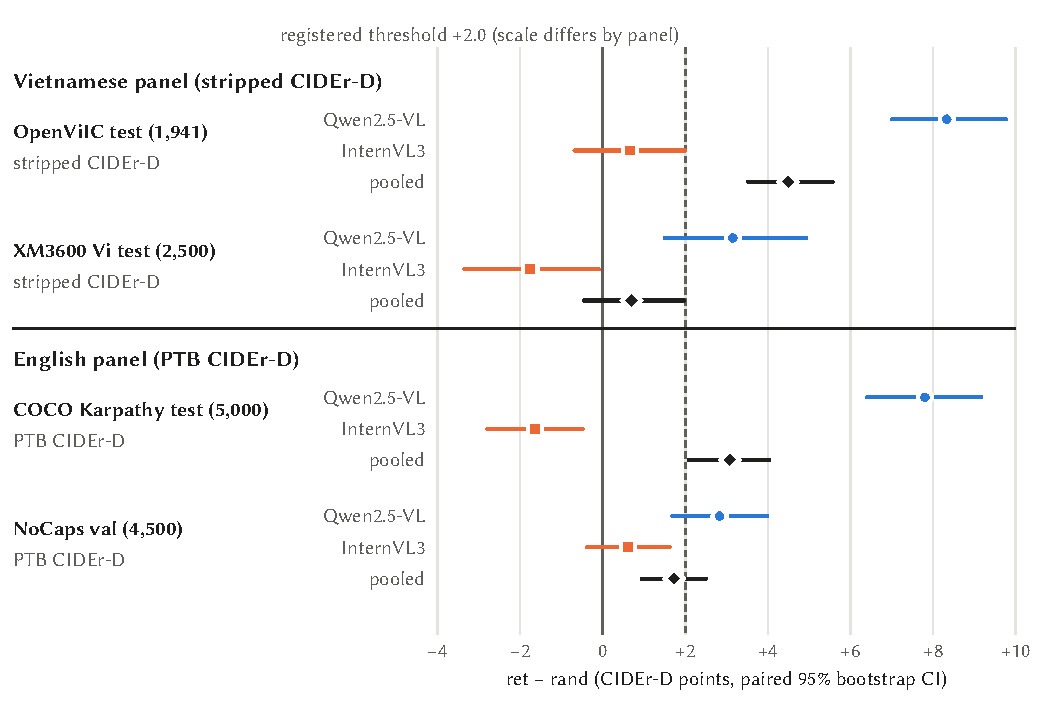
\includegraphics[keepaspectratio]{fig1_ret_minus_rand.pdf}}
\Description{Forest plot of ret minus rand differences with 95 percent confidence intervals for Qwen2.5-VL, InternVL3 and the pooled estimate on four test sets: OpenViIC test, XM3600 Vietnamese test, COCO Karpathy test and NoCaps val. A solid line marks zero and a dashed line the smallest effect of interest.}
\caption{\texttt{ret} − \texttt{rand} on the four scored sets, per backbone and pooled, with paired
95\% bootstrap CIs (values from Tables 7, 8 and 11; InternVL3 at its frozen τ = 0.10). Pooled rows
are the registered estimands (P1, XM-a, P1-EN, S-NC); per-backbone rows are reported rows.
Vietnamese sets use stripped CIDEr-D and English sets PTB CIDEr-D, in separate panels; no
cross-language difference is computed. Solid line: zero; dashed line: the registered +2.0, a
different quantity on each scale.}
\end{figure}

\textbf{The registered verdicts in each language} (Figure 1). In each language the registered
in-domain prediction passed: P1 on OpenViIC test (+4.49 {[}3.52, 5.57{]}, stripped CIDEr-D) and
P1-EN on COCO Karpathy test (+3.08 {[}2.08, 4.03{]}, PTB CIDEr-D). In each language the registered
prediction on a set outside the memory's source did not pass, but the two failures differ: on XM3600
Vietnamese the gain was not detected (XM-a FAIL, CI including zero); on NoCaps val the CI lies above
zero and the point is below the SESOI, under a stricter rule (S-NC FAIL). Within each language the
in-domain gain is carried by Qwen2.5-VL. The InternVL3 rows differ between the languages: not
detected on OpenViIC test, and below zero on COCO.

\textbf{A post-hoc question: does retrieval help mainly when the memory covers the target domain?}
The Vietnamese memory holds no XM3600 captions, and the pooled gain was not detected there. The
English memory is COCO, and on NoCaps the point estimate is largest for the images whose objects are
all COCO classes and smallest for those with none (Table 12). Both observations are compatible with
the hypothesis that retrieved examples beat random ones when the memory holds captions of images
like the query. A text-only retrieval stage in a different pipeline, for Indigenous languages of the
Americas, also helped only with large in-domain corpora \citep{Dhawan2026Gators}. The hypothesis was
not registered and is not tested here. Three observations limit it:

\begin{enumerate}
\def\labelenumi{\arabic{enumi}.}
\tightlist
\item
  \textbf{The domain split has overlapping CIs.} The three NoCaps domains were reported, not
  compared.
\item
  \textbf{Image-level similarity did not order the gain.} Within OpenViIC test the gain did not rise
  monotonically with the nearest-neighbour cosine, and within XM-test2500 the high-cosine tertile
  had the lowest point (Section 6.5).
\item
  \textbf{For Qwen2.5-VL the gain shrinks rather than vanishes.} Its out-of-source rows stay above
  zero: +3.15 {[}1.50, 4.93{]} on XM-test2500 and +2.83 {[}1.69, 3.98{]} on NoCaps val (reported
  rows). The pooled failures also reflect InternVL3's rows.
\end{enumerate}

The development-set memory-size ablation of Section 6.8 is consistent with this reading (a smaller
in-domain memory gave a smaller gain); it is dev evidence and does not test the English rows.

\subsection{Disclosures for the English arm}\label{disclosures-for-the-english-arm}

\textbf{When the registration was written.} The registration was drafted after the three Vietnamese
decision files had been read (Section 7.4), but its sets, SESOI, arms and configuration had been
fixed in an earlier ruling, before any Vietnamese verdict; only the NoCaps rule followed XM-a. It
was committed before any English image was decoded, embedded or scored, and each set was decided
once (supplement, ``Test-run operations'').

\textbf{The English deletion step is a port.} InternVL3's τ = 0.10 was selected on Vietnamese
development data with the Vietnamese object matcher. The English side uses the companion
object-precision study's COCO-80 matcher, which shares 24 of its 80 classes with the 112-class
Vietnamese verifier map, and a mechanical class phrase. Its calibration is untested in English, so
the τ = −∞ row is printed beside every τ = 0.10 row.

\textbf{Image source and earlier contact.} NoCaps images were fetched by their official Open Images
ids from the Open Images validation bucket, because the NoCaps proxy no longer serves them; bytes or
resolution may differ. Earlier contact with the English sets (a companion study's scoring on the
Karpathy test, an earlier zero-shot decode of 295 Karpathy test images, another study's 1,000 NoCaps
images, and the 133 Karpathy test images in the UIT-ViIC pre-check of Section 7.2) is listed in the
supplement. None of those outputs is reused here, and no design choice follows from them.

\textbf{Compute.} The two test blocks used 6.33 (COCO) and 6.88 (NoCaps) GPU-hours, together 13.22
of the 25 GPU-hour test cap, on one 24 GB GPU.

\subsection{Context from published systems (no ordering
implied)}\label{context-from-published-systems-no-ordering-implied}

Table S15 prints the CIDEr scores that other papers report on the benchmarks of this study beside
this study's own runs, with its inclusion rule and each system's setting and data. It is not a
ranking: scorers, tokenisation, document-frequency sets, memories, image subsets and, for
Vietnamese, word segmentation differ between papers, and no test set of this study was re-scored
with a published scorer. The one reading it supports is that a training-free prompt remains far
below a fine-tuned system on OpenViIC test (best published baseline 75.58 CIDEr
\citep{Bui2023OpenViIC}), which is the gap that motivates retrieval (Section 1).

\section{Limitations and threats to validity}\label{limitations-and-threats-to-validity}

\subsection{Limitations}\label{limitations}

\begin{itemize}
\tightlist
\item
  \textbf{Two backbones, and the effect is carried by one.} In both languages the in-domain gain is
  carried mainly by Qwen2.5-VL. For InternVL3 the gain was not detected on OpenViIC test, and on
  COCO its row is below zero (−1.64 {[}−2.79, −0.49{]}). The dev-only ablations of Section 6.8 trace
  part of this dependence to the frozen deletion step, but outside in-domain Vietnamese InternVL3's
  τ = −∞ row is not detected either (XM-test2500, COCO, NoCaps). With two backbones, the study
  cannot say which property of a model predicts the gain. The pooled estimand averages two
  backbone-plus-configuration pairs that differ in k, order, tail and τ, so it is not an effect for
  a typical MLLM.
\item
  \textbf{Out of the memory's source, the registered predictions did not pass.} On XM3600 Vietnamese
  the gain was not detected (XM-a FAIL). On NoCaps val the CI lies above zero but the point stayed
  below the SESOI (S-NC FAIL), under a rule that was fixed after XM-a was known and is stricter than
  XM-a's. Neither memory holds captions of the target set. Memory source and test set change
  together across these rows, and no test varied the memory on fixed test images, so the source
  match is confounded with the test set. The ``domain coverage'' reading of Section 8.4 is post hoc
  and untested, and its per-domain rows have overlapping CIs.
\item
  \textbf{The metric is reference-based.} CIDEr-D rewards matching the references' wording. In
  Vietnamese, the stripped column removes the trailing-period effect, and the PTB column agrees with
  it. Still, part of any \texttt{ret} − \texttt{rand} gain may be closer wording of image-specific
  content rather than better content. The study has no human judgments; by design, it uses existing
  data and labels only.
\item
  \textbf{Object measures depend on the matcher and the gold.} On OpenViIC, gold objects come from
  the union of the references, so a correct object that no reference names counts as an error. On
  XM3600, the verified labels cover only the mapped classes. The English arm registered no
  object-precision prediction.
\item
  \textbf{The memory and test sets come from related sources.} KTVIC and OpenViIC share images. We
  removed byte-identical and near-duplicate images between the memory and every protected set, and
  excluded the near-duplicates of the tuning set from the primary set. Overlaps below the pixel
  rule's thresholds would not be caught. The same rule protected the English sets.
\item
  \textbf{One test look, one machine, one run, one random draw.} Each test set was decoded once with
  greedy decoding. The CIs capture image sampling conditional on one seeded \texttt{rand} assignment
  per image and on full-set document frequencies; they do not include the variation from drawing
  other random examples, or run-to-run variation. Decode-parity checks on the same machine and
  software stack found no run-to-run variation on development data (52/52 identical captions per
  backbone; supplement, ``Test-run operations'', and Table S14).
\item
  \textbf{The backbones' training data are not fully disclosed.} The Qwen2.5-VL report
  \citep{Bai2025Qwen25VL} describes its training data by category (image captions, interleaved
  image-text, OCR data that include Vietnamese); in our reading it does not name COCO, NoCaps or a
  Vietnamese caption set. The InternVL3 report \citep{Zhu2025InternVL3} builds on the corpora of
  InternVL2.5, whose report lists COCO captions, Open Images captions and TextCaps among its
  training data \citep{Chen2024InternVL25}. COCO images and captions, and Open Images images like
  those of NoCaps, may therefore have been seen in training, at least by InternVL3. The equal-k
  \texttt{rand} control removes contamination that \texttt{ret} and \texttt{rand} share, but not
  contamination that interacts with retrieval (retrieved captions cueing memorised references).
  ``Training-free'' means no task training in this study; this is a desk check of public reports,
  not an audit.
\item
  \textbf{No priority claim.} Retrieval in-context captioning has been studied before (Section 2).
  This paper's contribution is the controlled, preregistered comparison, not the method.
\end{itemize}

\subsection{Threats to validity}\label{threats-to-validity}

\textbf{Internal validity.} \texttt{ret}, \texttt{rand} and \texttt{fix} share one prompt template,
one k and one decoder, and differ only in which captions are shown; \texttt{rand} is seeded per
image. Rule L did not fire on OpenViIC test (0.074, 0.039) or COCO (0.019, 0.019), and the
source-dataset share of shown examples is near one for every arm (Table S6), so the contrast is not
between in-domain and out-of-domain style. One threat remains, a design limitation of the registered
estimand: InternVL3's deletion step acts after decoding and treats \texttt{ret} and \texttt{rand}
captions differently, because they introduce different numbers of neighbour-only objects (Section
6.8). On OV-test it lowered CIDEr-D and did not improve CHAIR\_i or ΔP\_cm (Section 6.6); the
registered τ = −∞ secondary is printed beside every τ = 0.10 row for this reason.

\textbf{Construct validity.} CIDEr-D measures agreement with the references, in Vietnamese on
word-segmented text and in English on PTB tokens; the two scales are not comparable. Count-matched
object precision guards against a gain bought by copying wrong objects; it held for both backbones
on OpenViIC test and was not registered in English.

\textbf{External validity.} The result applies in domain, on two benchmarks in two languages, with
two 7--8B open MLLMs and a memory of one or two benchmarks' training captions. It does not apply out
of the memory's source (XM3600, NoCaps), and it is untested for other model families or sizes,
sampled decoding or prompts with example images. The English arm reused Vietnamese-chosen
configurations, so it is a conservative transfer test, not an estimate of the best English setting.

\textbf{Statistical conclusion validity and researcher degrees of freedom.} Every decision uses a
registered rule on a paired image bootstrap with a fixed SESOI that was a planning value, carried to
English without recalibration (Sections 5.2 and 5.4). Per-backbone, per-domain and development rows
carry unadjusted CIs and no claim, and no p-values are reported. Configurations were frozen on
development data and each test set was looked at once. Three choices were made with knowledge of
earlier results and are disclosed (Sections 6.8, 7.4 and 8.5): the English registration followed the
Vietnamese verdicts, the stricter NoCaps rule followed XM-a, and two of the six ablation τ points
were known.

\subsection{Reproducibility}\label{reproducibility}

Every model snapshot, processor setting, environment, prompt template, list and code file is pinned
by sha256, and each decision file records the hashes of the ledgers it read, the registration hash
and the code commit. Scores, image ids and hashes are released; captions, example files, embeddings
and per-image ledgers are not. A third party can re-run the study from the public datasets with the
released code, lists and seeds on one 24 GB GPU (9.59 GPU-hours for the Vietnamese test, 13.22 for
the English one) and check each run against the released hashes.

\section{Conclusion}\label{conclusion}

We asked whether retrieved example captions help two open MLLMs caption images more than random
captions from the same memory. We asked it first in Vietnamese and then, with the same frozen
configurations and no re-tuning, in English. Each question was answered by a preregistered study
with one look per test set.

\textbf{In domain, in both languages.} On the OpenViIC test, retrieval beat random examples by +4.49
{[}3.52, 5.57{]} stripped CIDEr-D points pooled, P1 PASS. On the COCO Karpathy test it did so by
+3.08 {[}2.08, 4.03{]} PTB CIDEr-D points, P1-EN PASS. In both languages the gain is carried mainly
by Qwen2.5-VL; InternVL3's row is not detected on OpenViIC test and, as a reported row, below zero
on COCO. On OpenViIC test, neither model lost count-matched object precision against its own
zero-shot captions; this compares the full in-context prompt with zero-shot, not retrieved with
random examples.

\textbf{Outside the memory's source.} On XM3600 Vietnamese the gain was not detected (+0.70
{[}−0.45, 1.97{]}), and the registered XM3600 prediction is not confirmed. On NoCaps val the pooled
gain was +1.73 {[}0.94, 2.50{]}: its CI lies above zero, but the point is below the SESOI under the
stricter English rule (S-NC FAIL), so the transfer claim is not made. Its reported per-domain rows
fall from the images with only COCO classes to those with none.

\textbf{Controls.} In domain, the registered S-zf row puts \texttt{ret} − \texttt{zs} at +14.30
{[}13.38, 15.24{]}, against P1's \texttt{ret} − \texttt{rand} of +4.49 {[}3.52, 5.57{]};
descriptively, random in-domain examples already score well above zero-shot (Table 6).

\textbf{What a practitioner can take from this.} Three things are needed before a gain over
zero-shot is attributed to retrieval:

\begin{enumerate}
\def\labelenumi{\arabic{enumi}.}
\tightlist
\item
  a random-example control at equal k, drawn from the same memory;
\item
  the result for each backbone, not only the pooled one;
\item
  to consider whether the memory's captions come from the target set's source. In this study the
  registered predictions passed only there, but memory source and test set changed together, and
  Qwen2.5-VL's out-of-source rows stayed above zero, so this is an observation and not a tested
  cause.
\end{enumerate}

A post-decode deletion step needs the same care: on the development set it removed more from
retrieved-example captions than from random ones (Section 6.8).

\textbf{Data and code availability.} We release:

\begin{itemize}
\tightlist
\item
  the registrations, with their pinned lists;
\item
  the test code and the decision files;
\item
  scores, image ids and sha256 hashes.
\end{itemize}

No caption from any dataset, no model caption and no per-image ledger is released. The authors of
UIT-OpenViIC and KTVIC confirmed in writing (2026-10-28) the use of their datasets in this study;
the confirmations are on file with the corresponding author. UIT-ViIC is not used as data; it
appears only as aggregate counts and image-id pointers (Section 7.2), no UIT-ViIC caption or
per-image panel is shown or released, and no permission from its authors is claimed. {[}Repository
link and archive DOI withheld for anonymous review; an anonymised copy of the registrations, code
and decision files can be provided to the editor.{]}

\begin{acks}
\textbf{Use of generative AI.} During this work the authors used AI-assisted tools (a large language
model coding and writing assistant) to help write analysis scripts, check consistency between the
text and the recorded results, verify bibliographic identifiers, and draft and edit text. The
authors reviewed and edited all content and take full responsibility for it.
\end{acks}

\bibliographystyle{ACM-Reference-Format}\bibliography{paperC}
\end{document}
